% Options for packages loaded elsewhere
\PassOptionsToPackage{unicode}{hyperref}
\PassOptionsToPackage{hyphens}{url}
\PassOptionsToPackage{dvipsnames,svgnames,x11names}{xcolor}
%
\documentclass[
  letterpaper,
]{book}

\usepackage{amsmath,amssymb}
\usepackage{iftex}
\ifPDFTeX
  \usepackage[T1]{fontenc}
  \usepackage[utf8]{inputenc}
  \usepackage{textcomp} % provide euro and other symbols
\else % if luatex or xetex
  \usepackage{unicode-math}
  \defaultfontfeatures{Scale=MatchLowercase}
  \defaultfontfeatures[\rmfamily]{Ligatures=TeX,Scale=1}
\fi
\usepackage{lmodern}
\ifPDFTeX\else  
    % xetex/luatex font selection
\fi
% Use upquote if available, for straight quotes in verbatim environments
\IfFileExists{upquote.sty}{\usepackage{upquote}}{}
\IfFileExists{microtype.sty}{% use microtype if available
  \usepackage[]{microtype}
  \UseMicrotypeSet[protrusion]{basicmath} % disable protrusion for tt fonts
}{}
\makeatletter
\@ifundefined{KOMAClassName}{% if non-KOMA class
  \IfFileExists{parskip.sty}{%
    \usepackage{parskip}
  }{% else
    \setlength{\parindent}{0pt}
    \setlength{\parskip}{6pt plus 2pt minus 1pt}}
}{% if KOMA class
  \KOMAoptions{parskip=half}}
\makeatother
\usepackage{xcolor}
\setlength{\emergencystretch}{3em} % prevent overfull lines
\setcounter{secnumdepth}{5}
% Make \paragraph and \subparagraph free-standing
\ifx\paragraph\undefined\else
  \let\oldparagraph\paragraph
  \renewcommand{\paragraph}[1]{\oldparagraph{#1}\mbox{}}
\fi
\ifx\subparagraph\undefined\else
  \let\oldsubparagraph\subparagraph
  \renewcommand{\subparagraph}[1]{\oldsubparagraph{#1}\mbox{}}
\fi


\providecommand{\tightlist}{%
  \setlength{\itemsep}{0pt}\setlength{\parskip}{0pt}}\usepackage{longtable,booktabs,array}
\usepackage{calc} % for calculating minipage widths
% Correct order of tables after \paragraph or \subparagraph
\usepackage{etoolbox}
\makeatletter
\patchcmd\longtable{\par}{\if@noskipsec\mbox{}\fi\par}{}{}
\makeatother
% Allow footnotes in longtable head/foot
\IfFileExists{footnotehyper.sty}{\usepackage{footnotehyper}}{\usepackage{footnote}}
\makesavenoteenv{longtable}
\usepackage{graphicx}
\makeatletter
\def\maxwidth{\ifdim\Gin@nat@width>\linewidth\linewidth\else\Gin@nat@width\fi}
\def\maxheight{\ifdim\Gin@nat@height>\textheight\textheight\else\Gin@nat@height\fi}
\makeatother
% Scale images if necessary, so that they will not overflow the page
% margins by default, and it is still possible to overwrite the defaults
% using explicit options in \includegraphics[width, height, ...]{}
\setkeys{Gin}{width=\maxwidth,height=\maxheight,keepaspectratio}
% Set default figure placement to htbp
\makeatletter
\def\fps@figure{htbp}
\makeatother
\newlength{\cslhangindent}
\setlength{\cslhangindent}{1.5em}
\newlength{\csllabelwidth}
\setlength{\csllabelwidth}{3em}
\newlength{\cslentryspacingunit} % times entry-spacing
\setlength{\cslentryspacingunit}{\parskip}
\newenvironment{CSLReferences}[2] % #1 hanging-ident, #2 entry spacing
 {% don't indent paragraphs
  \setlength{\parindent}{0pt}
  % turn on hanging indent if param 1 is 1
  \ifodd #1
  \let\oldpar\par
  \def\par{\hangindent=\cslhangindent\oldpar}
  \fi
  % set entry spacing
  \setlength{\parskip}{#2\cslentryspacingunit}
 }%
 {}
\usepackage{calc}
\newcommand{\CSLBlock}[1]{#1\hfill\break}
\newcommand{\CSLLeftMargin}[1]{\parbox[t]{\csllabelwidth}{#1}}
\newcommand{\CSLRightInline}[1]{\parbox[t]{\linewidth - \csllabelwidth}{#1}\break}
\newcommand{\CSLIndent}[1]{\hspace{\cslhangindent}#1}

\makeatletter
\@ifpackageloaded{tcolorbox}{}{\usepackage[skins,breakable]{tcolorbox}}
\@ifpackageloaded{fontawesome5}{}{\usepackage{fontawesome5}}
\definecolor{quarto-callout-color}{HTML}{909090}
\definecolor{quarto-callout-note-color}{HTML}{0758E5}
\definecolor{quarto-callout-important-color}{HTML}{CC1914}
\definecolor{quarto-callout-warning-color}{HTML}{EB9113}
\definecolor{quarto-callout-tip-color}{HTML}{00A047}
\definecolor{quarto-callout-caution-color}{HTML}{FC5300}
\definecolor{quarto-callout-color-frame}{HTML}{acacac}
\definecolor{quarto-callout-note-color-frame}{HTML}{4582ec}
\definecolor{quarto-callout-important-color-frame}{HTML}{d9534f}
\definecolor{quarto-callout-warning-color-frame}{HTML}{f0ad4e}
\definecolor{quarto-callout-tip-color-frame}{HTML}{02b875}
\definecolor{quarto-callout-caution-color-frame}{HTML}{fd7e14}
\makeatother
\makeatletter
\makeatother
\makeatletter
\@ifpackageloaded{bookmark}{}{\usepackage{bookmark}}
\makeatother
\makeatletter
\@ifpackageloaded{caption}{}{\usepackage{caption}}
\AtBeginDocument{%
\ifdefined\contentsname
  \renewcommand*\contentsname{Table of contents}
\else
  \newcommand\contentsname{Table of contents}
\fi
\ifdefined\listfigurename
  \renewcommand*\listfigurename{List of Figures}
\else
  \newcommand\listfigurename{List of Figures}
\fi
\ifdefined\listtablename
  \renewcommand*\listtablename{List of Tables}
\else
  \newcommand\listtablename{List of Tables}
\fi
\ifdefined\figurename
  \renewcommand*\figurename{Figure}
\else
  \newcommand\figurename{Figure}
\fi
\ifdefined\tablename
  \renewcommand*\tablename{Table}
\else
  \newcommand\tablename{Table}
\fi
}
\@ifpackageloaded{float}{}{\usepackage{float}}
\floatstyle{ruled}
\@ifundefined{c@chapter}{\newfloat{codelisting}{h}{lop}}{\newfloat{codelisting}{h}{lop}[chapter]}
\floatname{codelisting}{Listing}
\newcommand*\listoflistings{\listof{codelisting}{List of Listings}}
\makeatother
\makeatletter
\@ifpackageloaded{caption}{}{\usepackage{caption}}
\@ifpackageloaded{subcaption}{}{\usepackage{subcaption}}
\makeatother
\makeatletter
\@ifpackageloaded{tcolorbox}{}{\usepackage[skins,breakable]{tcolorbox}}
\makeatother
\makeatletter
\@ifundefined{shadecolor}{\definecolor{shadecolor}{HTML}{31BAE9}}
\makeatother
\makeatletter
\makeatother
\makeatletter
\@ifpackageloaded{sidenotes}{}{\usepackage{sidenotes}}
\@ifpackageloaded{marginnote}{}{\usepackage{marginnote}}
\makeatother
\makeatletter
\makeatother
\ifLuaTeX
\usepackage[bidi=basic]{babel}
\else
\usepackage[bidi=default]{babel}
\fi
\babelprovide[main,import]{american}
% get rid of language-specific shorthands (see #6817):
\let\LanguageShortHands\languageshorthands
\def\languageshorthands#1{}
\ifLuaTeX
  \usepackage{selnolig}  % disable illegal ligatures
\fi
\IfFileExists{bookmark.sty}{\usepackage{bookmark}}{\usepackage{hyperref}}
\IfFileExists{xurl.sty}{\usepackage{xurl}}{} % add URL line breaks if available
\urlstyle{same} % disable monospaced font for URLs
\hypersetup{
  pdftitle={Through the Looking Glass},
  pdfauthor={Curtis M. Lively},
  pdflang={en-US},
  colorlinks=true,
  linkcolor={blue},
  filecolor={Maroon},
  citecolor={Blue},
  urlcolor={Blue},
  pdfcreator={LaTeX via pandoc}}

\title{Through the Looking Glass}
\usepackage{etoolbox}
\makeatletter
\providecommand{\subtitle}[1]{% add subtitle to \maketitle
  \apptocmd{\@title}{\par {\large #1 \par}}{}{}
}
\makeatother
\subtitle{I. Why Cross-Fertilize?}
\author{Curtis M. Lively}
\date{17 October 2023}

\begin{document}
\frontmatter
\maketitle
\ifdefined\Shaded\renewenvironment{Shaded}{\begin{tcolorbox}[interior hidden, borderline west={3pt}{0pt}{shadecolor}, enhanced, breakable, frame hidden, sharp corners, boxrule=0pt]}{\end{tcolorbox}}\fi

\renewcommand*\contentsname{Contents}
{
\hypersetup{linkcolor=}
\setcounter{tocdepth}{2}
\tableofcontents
}
\listoffigures
\listoftables
\mainmatter
\bookmarksetup{startatroot}

\hypertarget{front-matter}{%
\chapter*{Front Matter}\label{front-matter}}
\addcontentsline{toc}{chapter}{Front Matter}

\markboth{Front Matter}{Front Matter}

\hypertarget{about}{%
\section*{About}\label{about}}
\addcontentsline{toc}{section}{About}

\markright{About}

The following pages represent the first volume of a book. The main goal
was to introduce the evolutionary problem of sexual reproduction, with a
focus on competition between sexual and asexual females. But I also
incorporated some ideas on genetic polymorphism and phenotypic
plasticity with the goal of exploring ``variation strategies'' more
generally. Finally, I tried to weave in some history of the field, along
with some philosophy of science.

\hypertarget{acknowledgements}{%
\section*{Acknowledgements}\label{acknowledgements}}
\addcontentsline{toc}{section}{Acknowledgements}

\markright{Acknowledgements}

I gratefully acknowledge helpful comments from Amrita Bhattacharya, Zoe
Dinges, Kara Million, Deanna Soper, Mike Wade, Jukka Jokela, Dorota
Paczesniak, Steve Howard, Lynda Delph, Clark Craddock, Robert
Vrijenhoek, Jan McKenzie, Mike Winterbourn, Stuart West, Oren Harman,
and especially Maurine Neiman and her lab group at the University of
Iowa. Additional comments are welcome by
\href{mailto:clively@indiana.edu}{email}.

Special thanks to Zoe Michelle Dinges (ZMD), who redrew the graphs and
contributed original illustrations. Many thanks also to Adam Mazel of
Indiana University Libraries for preparing the document for online
publication.

This project was supported by the NSF OPUS program for the synthesis of
biological research (DEB-1906465). I am also grateful to the Institute
for Advanced Study in Berlin (Wissenschaftskolleg zu Berlin) for my stay
as a ``partner'' during 2022-2023.

\hypertarget{copyright-and-license}{%
\section*{Copyright and License}\label{copyright-and-license}}
\addcontentsline{toc}{section}{Copyright and License}

\markright{Copyright and License}

Copyright Curtis M. Lively 2023

{Through the Looking Glass: I. Why Cross-Fertilize?} by Curtis M. Lively
is licensed under a Creative Commons Attribution 4.0 International
License.

\hypertarget{publisher-information}{%
\section*{Publisher Information}\label{publisher-information}}
\addcontentsline{toc}{section}{Publisher Information}

\markright{Publisher Information}

\href{https://libraries.indiana.edu/}{Indiana University Bloomington
Libraries}

\hypertarget{how-to-cite}{%
\section*{How to Cite}\label{how-to-cite}}
\addcontentsline{toc}{section}{How to Cite}

\markright{How to Cite}

Lively, C. M. (2023, June ??). Through the Looking Glass: I. Why
Cross-Fertilize? Indiana University Bloomington Libraries
https://doi.org/

\part{Part One: Why Cross-Fertilize?}

\hypertarget{sec-why-sex}{%
\chapter{Why Sex?}\label{sec-why-sex}}

\begin{figure}

{\centering 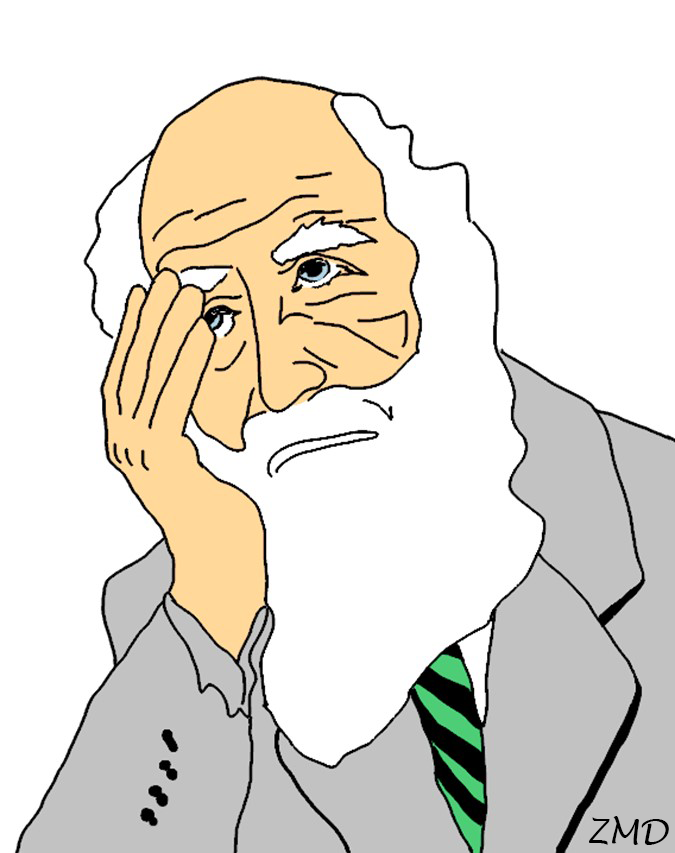
\includegraphics[width=0.4\textwidth,height=\textheight]{images/Picture1.png}

}

\end{figure}

\hypertarget{the-question}{%
\section{The Question}\label{the-question}}

Most PhD programs require that students pass a preliminary examination.
This was certainly true in my case. I was a PhD student at the
University of Arizona studying rocky intertidal communities in the
Northern Gulf of California. But the exams were not focused on our
research. They were ``depth-of-knowledge'' exams. My question from
Prof.~Astrid Kodric-Brown instructed me to read the preface of G.C.
Williams' book, \emph{Sex and Evolution}, which contains the following
text (Williams 1975): ``This book is written from a conviction that the
prevalence of sexual reproduction in higher plants and animals is
inconsistent with current evolutionary theory\ldots. Many well informed
readers may disagree with much of my reasoning, but I hope to at least
convince them that here is a crisis at hand in evolutionary
biology\ldots.''''

The question was something like this: \emph{Why does Williams think that
sexual reproduction poses a crisis for evolutionary biology, and what is
the solution}? A crisis? That was news to me. How could there be a
crisis on evolutionary biology 40-plus years after the modern synthesis?
My graduate course in theoretical population genetics did not mention
any crises. I was not convinced. And a little freaked out.

The structure of our exams was very loose. I don't remember having a
deadline to produce a written answer, but I do remember that I spent
several months on just this one question. During much of this time, I
was doing field work in Sonora, Mexico, sometimes under very harsh
conditions. But the more I studied the question, the more fascinated I
became. I came to think that there was, indeed, a very real anomaly
presented by sexual reproduction. Williams was right. Perhaps I was
especially interested in this anomaly because I had read Thomas Kuhn's
``The Structure of Scientific Revolutions'' as an undergraduate (Kuhn
1970). Kuhn made the case that dissecting anomalies can lead to
interesting advances, and that made sense to me. While I eventually
produced an essay to address the question, the answer felt incomplete. I
wanted to know more. There were many hypotheses, but there was no clear
general explanation. Many years later, I am still working on my prelim
question. This book is my revised answer.

\hypertarget{the-problem}{%
\section{The Problem}\label{the-problem}}

There are many problems with sexual reproduction, including the time
spent finding mates and the risk of contracting sexually transmitted
disease (review in Lehtonen et al.~2012). However, while important,
these costs do not form the core of the paradox. Historically, the
paradox of sex stems from two things: (1) the cost of meiosis, and (2)
the cost of producing males.

\hypertarget{the-cost-of-meiosis-reduced-relatedness}{%
\subsection{The cost of meiosis: reduced
relatedness}\label{the-cost-of-meiosis-reduced-relatedness}}

The ``cost of meiosis'' was proposed by George Williams (1975). His idea
was simply that females are only half as related to their outcrossed
offspring as they are to their self-fertilized or parthenogenetic
offspring.\footnote{I ran two years of field experiments designed to
  test for random settlement by genetically determined morphs. I also
  ran experiments designed to test for habitat selection by genetically
  determined morphs. The results were always negative. I finally tested
  for predator-induced development of the bent morph by placing
  \emph{Acanthina} snails in quadrats where juvenile barnacles had
  recently settled. I used herbivorous snails as a control. The results
  showed that the presence of \emph{Acanthina} induced development of
  the bent form, but the herbivorous snails did not. It was a thrilling
  discovery.} (See \protect\hyperlink{callout-1}{Box 1.1} for condensed
definitions.) Williams' idea also had theoretical support, as R.A.
Fisher had already shown that an allele causing self-fertilization would
rapidly spread to fixation, barring severe inbreeding depression (Fisher
1941). So, why cross-fertilize? The persistence of cross-fertilization
despite the cost of meiosis formed a paradox. This paradox created the
crisis that Williams saw in evolutionary biology.

\hypertarget{the-cost-of-males}{%
\subsection{The cost of males}\label{the-cost-of-males}}

The other way to look at the problem was proposed by John Maynard Smith
(Maynard Smith 1971, 1978). Here the issue is not relatedness. The
problem stems rather from the difference between sexuals and asexuals in
their per-capita birth rates (Figure~\ref{fig-1.1}). Imagine a
population of sexual individuals at carrying capacity (\(K_{sex}\)). At
\(K_{sex}\) the sexual females are, by definition, simply replacing
themselves. This means that each sexual female is, on average, producing
one son and one daughter. Both sons and daughters contribute genetically
to the next generation, but only females give birth. Now, consider a
mutation in a single female that causes her to reproduce asexually. She
gives birth to two daughters instead of one daughter and one son. These
two asexually produced daughters both give birth to two more daughters.
Hence, after just two generations, the asexual female has four
granddaughters, while the average sexual female has just one
granddaughter (Figure~\ref{fig-1.1}). This asymmetry should lead to the
rapid replacement of sexual females by asexual females
(Figure~\ref{fig-1-2}). And by ``rapid,'' I mean within tens of
generations, even for very large populations (Lively 1996). We thus seek
a selective force that can give an advantage to sexual reproduction on a
very short time scale.

\begin{figure}

\sidecaption{\label{fig-1.1}The cost of males. Imagine a single clonal
female in a sexual population at carrying capacity, \(K_{sex}\). At
\(K_{sex}\), the sexual females are, on average, producing one daughter
and one son. In contrast, the clonal female produces two daughters and
four granddaughters. Hence, the clonal lineage should rapidly eliminate
the sexual population (Figure~\ref{fig-1-2}). However, in nature,
asexual reproduction is very rare in both plants (Whitton et al.~2008)
and animals (Vrijenhoek 1998). Hence the paradox. Why is sexual
reproduction so costly and yet so common?}

{\centering 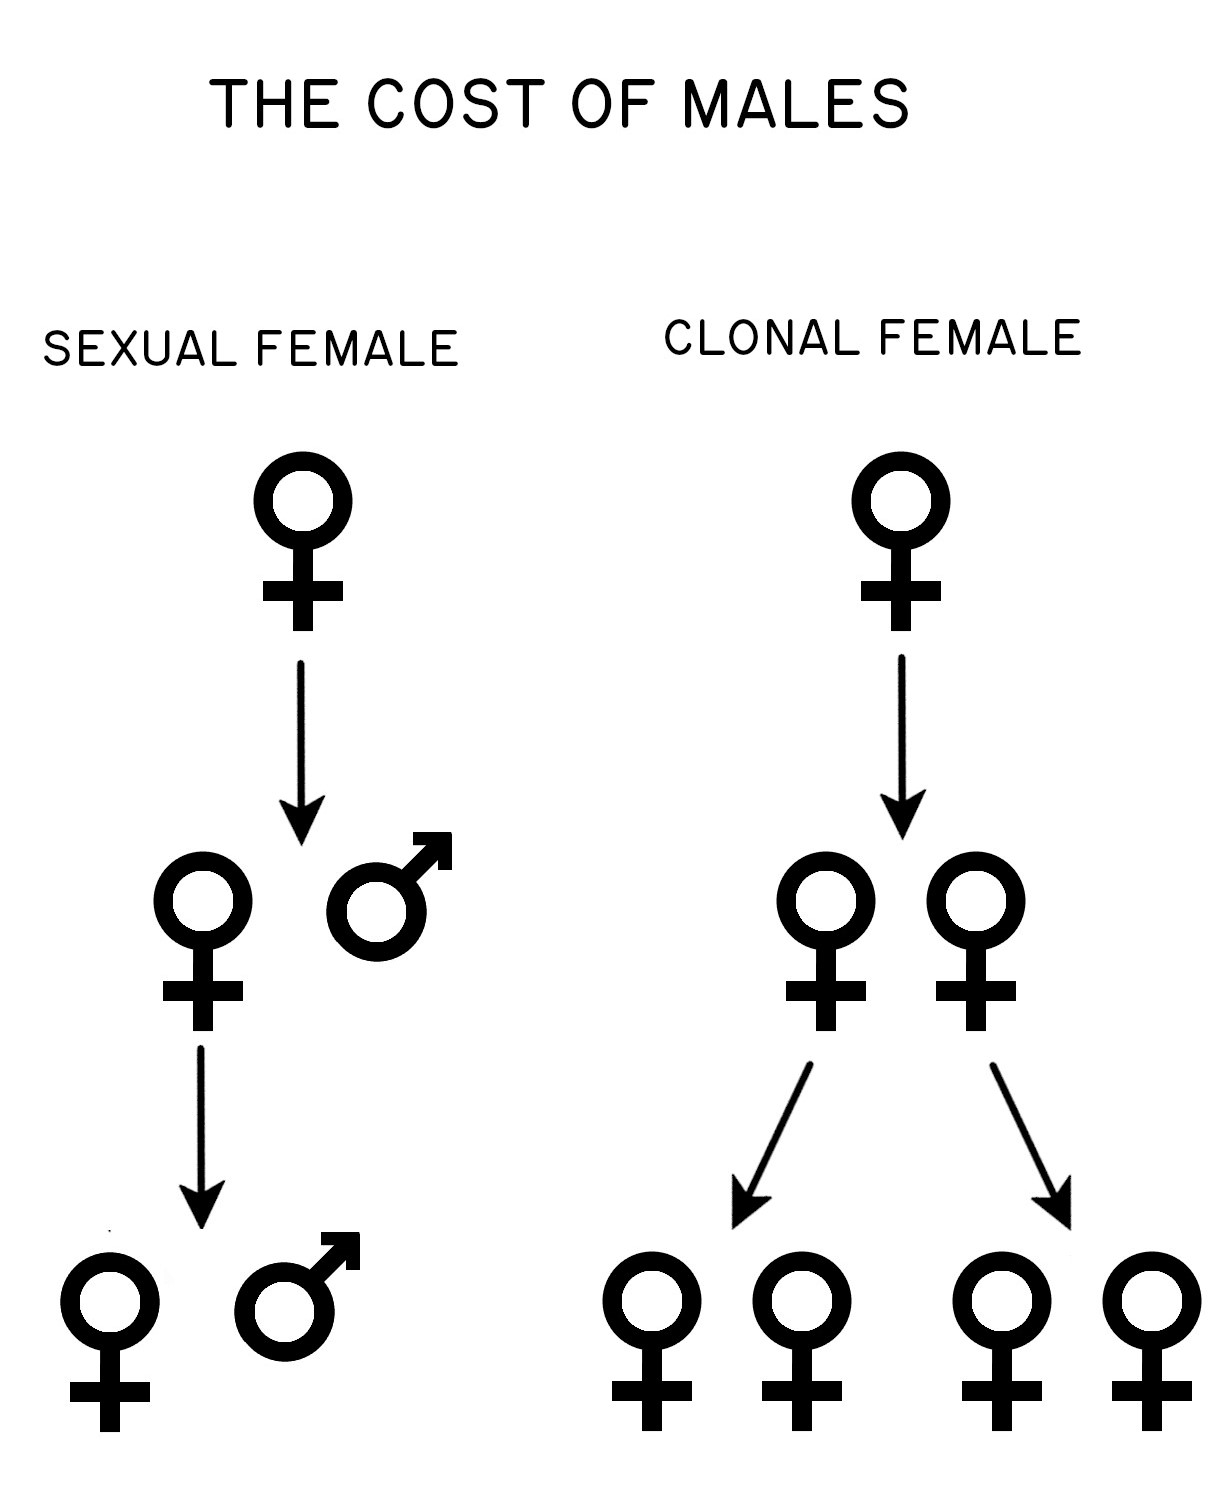
\includegraphics[width=0.75\textwidth,height=\textheight]{images/fig1-1.jpg}

}

\end{figure}

Several assumptions went into Maynard Smith\textquotesingle s model for
the cost of males. In particular, he assumed that sexual females and
asexual females make the same number of offspring, and that the
survivorship of these offspring is also the same. Maynard Smith referred
to this as the ``all-else-equal assumption.'' Unfortunately, some
authors have taken the phrase ``all-else-equal'' to mean that everything
else is exactly equal. But this is not the case. Maynard Smith did not
assume, for example, that sexuals and asexuals have the same ploidy
value.\footnote{Plasticity is more mainstream now than it was in the
  1980s. One reviewer of my paper was incredulous and recommended
  rejection from \emph{Evolution} because the bent morph was not
  ``genetically determined.'' The Associate Editor (John Endler)
  rejected the review and accepted the paper. Clearly, it is the
  developmental strategy that is genetically determined, not the morph
  per se (see also Lively et al.~2000, Hazel et al.~2004).} His model
only assumes that sexual and asexual females have equal fecundities and
survivorship probabilities (see \protect\hyperlink{callout-2}{Box 1.2}).
Under this assumption, a very rare clone would double in frequency in
the next generation. Maynard Smith called this doubling-when-rare the
two-fold cost of sex.

\hypertarget{contrasting-the-costs}{%
\subsection{Contrasting the costs}\label{contrasting-the-costs}}

The two alternative costs of sex raise an immediate question. Does the
cost of sex result from reduced relatedness between mother and
offspring, or from the cost of producing males? Or is the cost some
combination of both? These questions are not easy to answer; but there
is an algebraic solution, which suggests that the (1) two costs are
mutually exclusive and (2) that they apply to different kinds of
uniparental progeny (Lively and Lloyd 1990). Roughly speaking, I think
we can adopt the following rules for the purpose of this book. When
considering the spread of a rare allele that induces self-fertilization
in hermaphrodites, the appropriate cost is Williams' cost of meiosis.
Here we have a single population in which the selfing allele is under
positive selection because it has a transmission advantage. On the other
hand, when we consider the spread of a clone into an obligately sexual
population, we are dealing with competition between two different
reproductively isolated groups. One group (the sexuals) produces males,
which do not make offspring. The other group (asexuals) produces only
females. Here the cost of sex stems from producing males. But the two
costs do not combine. The cost of sex is not four-fold.

\hypertarget{fig-1-2}{}
{
\makeatletter
\def\LT@makecaption#1#2#3{%
  \noalign{\smash{\hbox{\kern\textwidth\rlap{\kern\marginparsep
  \parbox[t]{\marginparwidth}{%
    \footnotesize{%
      \vspace{(1.1\baselineskip)}
    #1{#2: }\ignorespaces #3}}}}}}%
    }
\makeatother

{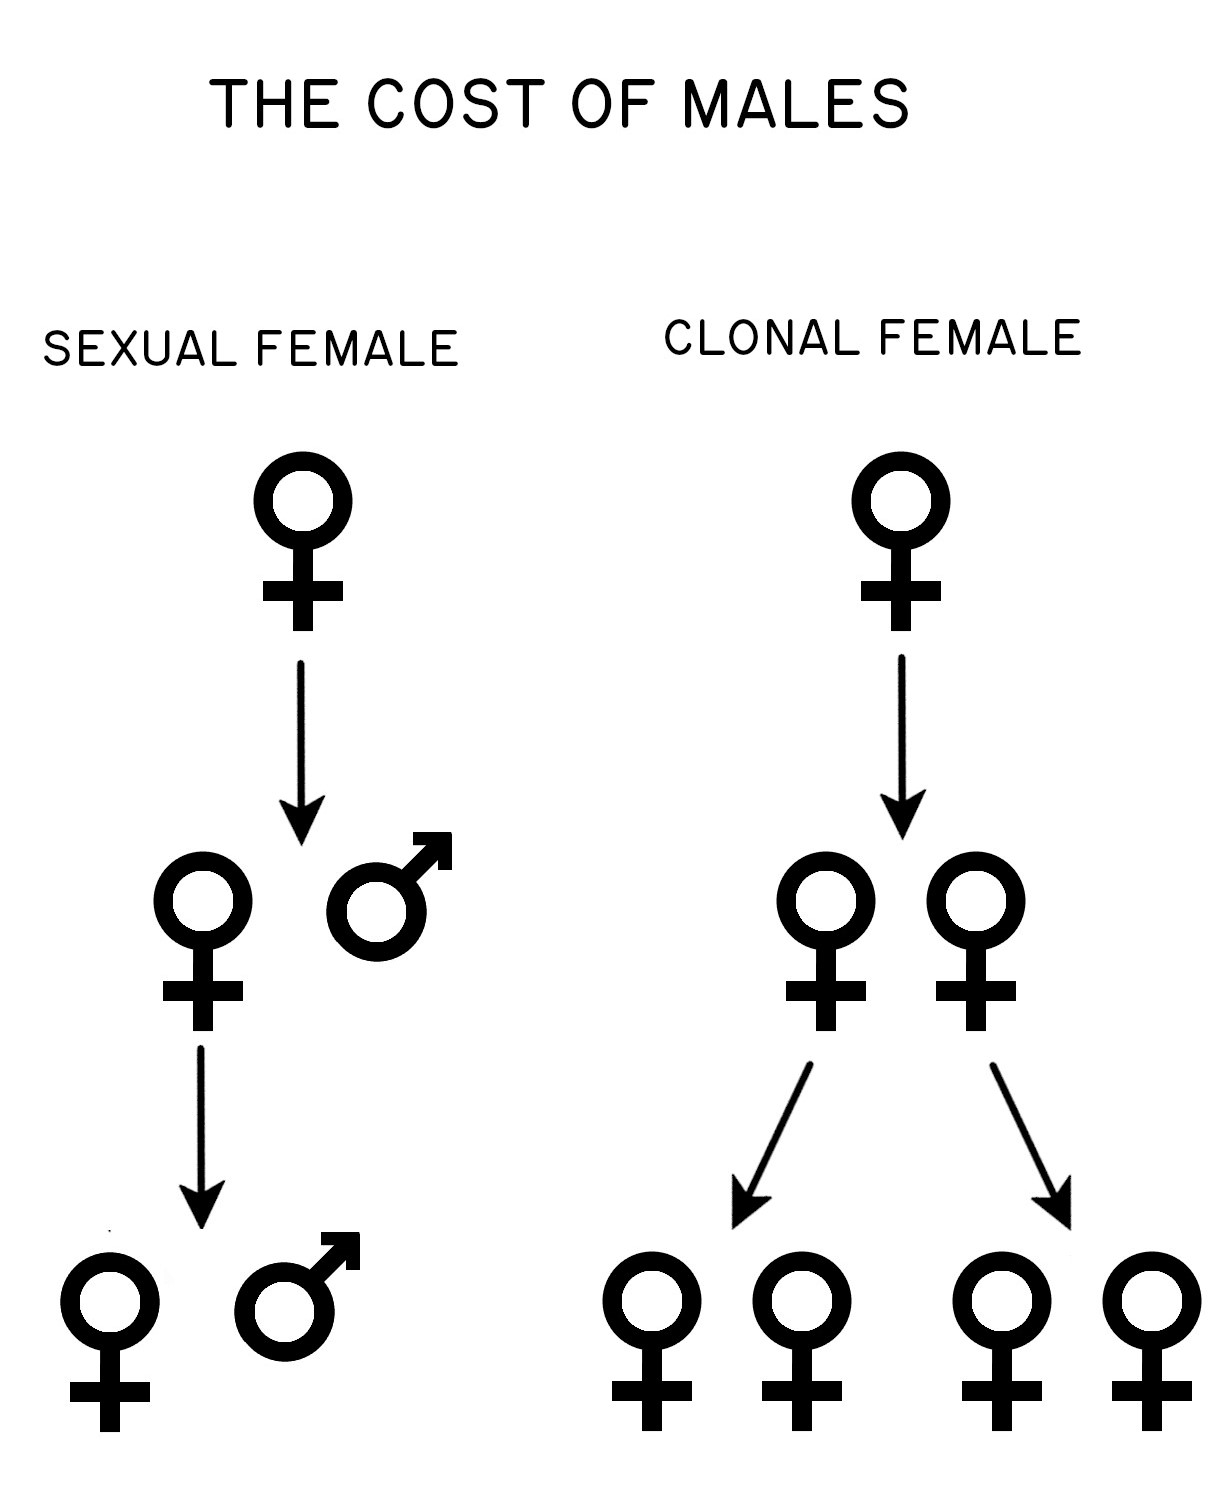
\includegraphics{images/fig1-2.jpg}}

\label{fig-1-2}Clonal invasion dynamics. Results from a simulation study
in which a single clonal individual was introduced into a sexual
population (Lively 2009b). \textbf{A} (top). Results for a 1:1 sex ratio
in the sexual population. Here the frequency of daughters produced by
sexual females was 1/2. The sexual population was initiated at carrying
capacity: \(K_{sex}\) = 10,000. A single parthenogenetic female was
introduced by the simulation at generation 1,000. Note that the asexual
lineage replaces the sexual population in about 25 generations, and that
it reaches a higher carrying capacity \(K_{asex}\) = 20,000. \textbf{B}
(bottom). Results for a female-biased sexual population. Here the
frequency of daughters produced by sexual females was 0.8. The sexual
population was initiated at carrying capacity: \(K_{sex}\) = 17,500. As
above, a single parthenogenetic female was introduced into the
population at generation 1,000. Note that the asexual lineage replaces
the sexual population, but it takes longer. The simulation assumes
annual reproduction and non-overlapping generations. The R code for the
simulation, including interactive graphical output, can be found
\href{https://raw.githubusercontent.com/IULibScholComm/through-the-looking-glass/main/sim\%20for\%20fig\%201.2(ZMD).R}{here}.
The interactive graph can also be run
\href{https://connect.posit.iu.edu/clonal-invasion-dynamics/}{here} for
users without R.

}

\hypertarget{the-cost-of-recombination}{%
\subsection{The cost of recombination}\label{the-cost-of-recombination}}

There is another paradox of sexual reproduction known as the ``cost of
recombination.'' Here the competition is not between sexual and asexual
females, or between outcrossing and selfing alleles, but rather between
alleles that modify the rate of recombination. So instead of asking
``Why cross-fertilize?'' we can assume cross-fertilization and ask,
``Why is there excess crossing-over during meiosis?'' Here is the
paradox. If combinations of alleles at different loci are favored by
natural selection (because together they create high-fitness offspring),
then recombination would break these favorable allelic combinations
apart. So, it makes no obvious sense to recombine more than needed for
normal meiosis. Indeed, Lewontin (1971) formally showed that:
\emph{\ldots{} the mean fitness of the population at equilibrium is a
maximum in the absence of recombination}.\footnote{Facultative
  parthenogenesis is used to mean environmentally cued production of
  parthenogenetic females. I was originally planning to work on a
  nematode population that produced a mixture of sexual males and
  females at high density but only parthenogenetic females at low
  density.} Hence, there are two interrelated anomalies:
cross-fertilization per se and meiotic recombination. Ideally, any
theory that explains the persistence of biparental sex could also solve
the paradox of recombination. But this need not be the case. They could
have different solutions.

\begin{tcolorbox}[enhanced jigsaw, left=2mm, bottomtitle=1mm, opacitybacktitle=0.6, breakable, leftrule=.75mm, coltitle=black, titlerule=0mm, opacityback=0, arc=.35mm, colback=white, title=\textcolor{quarto-callout-tip-color}{\faLightbulb}\hspace{0.5em}{Box 1.1}, toprule=.15mm, rightrule=.15mm, bottomrule=.15mm, colframe=quarto-callout-tip-color-frame, toptitle=1mm, colbacktitle=quarto-callout-tip-color!10!white]

\textbf{Short definitions of terms as used in this book. These
definitions do not include all possible nuances.}

\textbf{Carrying capacity.} The population density at which females have
just enough food to replace themselves. Sexual females must make two
offspring to replace themselves (assuming a 1:1 sex ratio), while
asexual females must only produce one offspring. Hence, asexuals should
have higher carrying capacities, as shown in (Figure~\ref{fig-1-2}).

\textbf{Cost of males}. The reduction in the per-capita growth rate of
sexual populations due to the production of males. The cost of males is
the appropriate cost for considering sexual subpopulations in
competition with obligately asexual subpopulations.

\textbf{Cost of meiosis}. The reduction in relatedness between mother
and offspring due to outcrossing. The cost of meiosis is the appropriate
cost for considering the spread of alleles that induce
self-fertilization.

\textbf{Clone}. A lineage of parthenogenetic females descended from the
same asexual female. Members of the same clone may have small genetic
differences, which accumulate by mutation over time.

\textbf{Cross-fertilization}. The exchange of gametes between different
individuals, which may or may not be related.

\textbf{Outcrossing}. A form of cross-fertilization, which specifies
crossing between unrelated individuals.

\textbf{Parthenogenesis}. Any form of asexual reproduction through ova.

\textbf{Recombination}. Genetic exchange between homologous chromosomes
during meiosis, especially when the exchange leads to gametes with
allele combinations not represented on the parental chromosomes.

\textbf{Self-fertilization}. The fusion of gametes from the same
individual.

\textbf{Sex/rec}. Shorthand for sexual reproduction and recombination.

\textbf{Sexual reproduction}. I use the term here to mean
cross-fertilization between unrelated individuals. However, the term is
more general, and can be used to mean the incorporation of novel genetic
material by any mechanism.

\end{tcolorbox}

\begin{figure}

\sidecaption{\label{fig-1.3}Two flower morphs (distyly) in
\emph{Primula}. Darwin found that the short-styled morph (left) is
incompatible with other short-style morphs, and that the long styled
morph (right) is incompatible with other long-style morphs. But the two
different morphs can cross-fertilize. The arrows show movement of pollen
from anthers to stigmas. The ``X'' indicates incompatibility. Redrawn
from Darwin (1862) by ZMD.}

{\centering 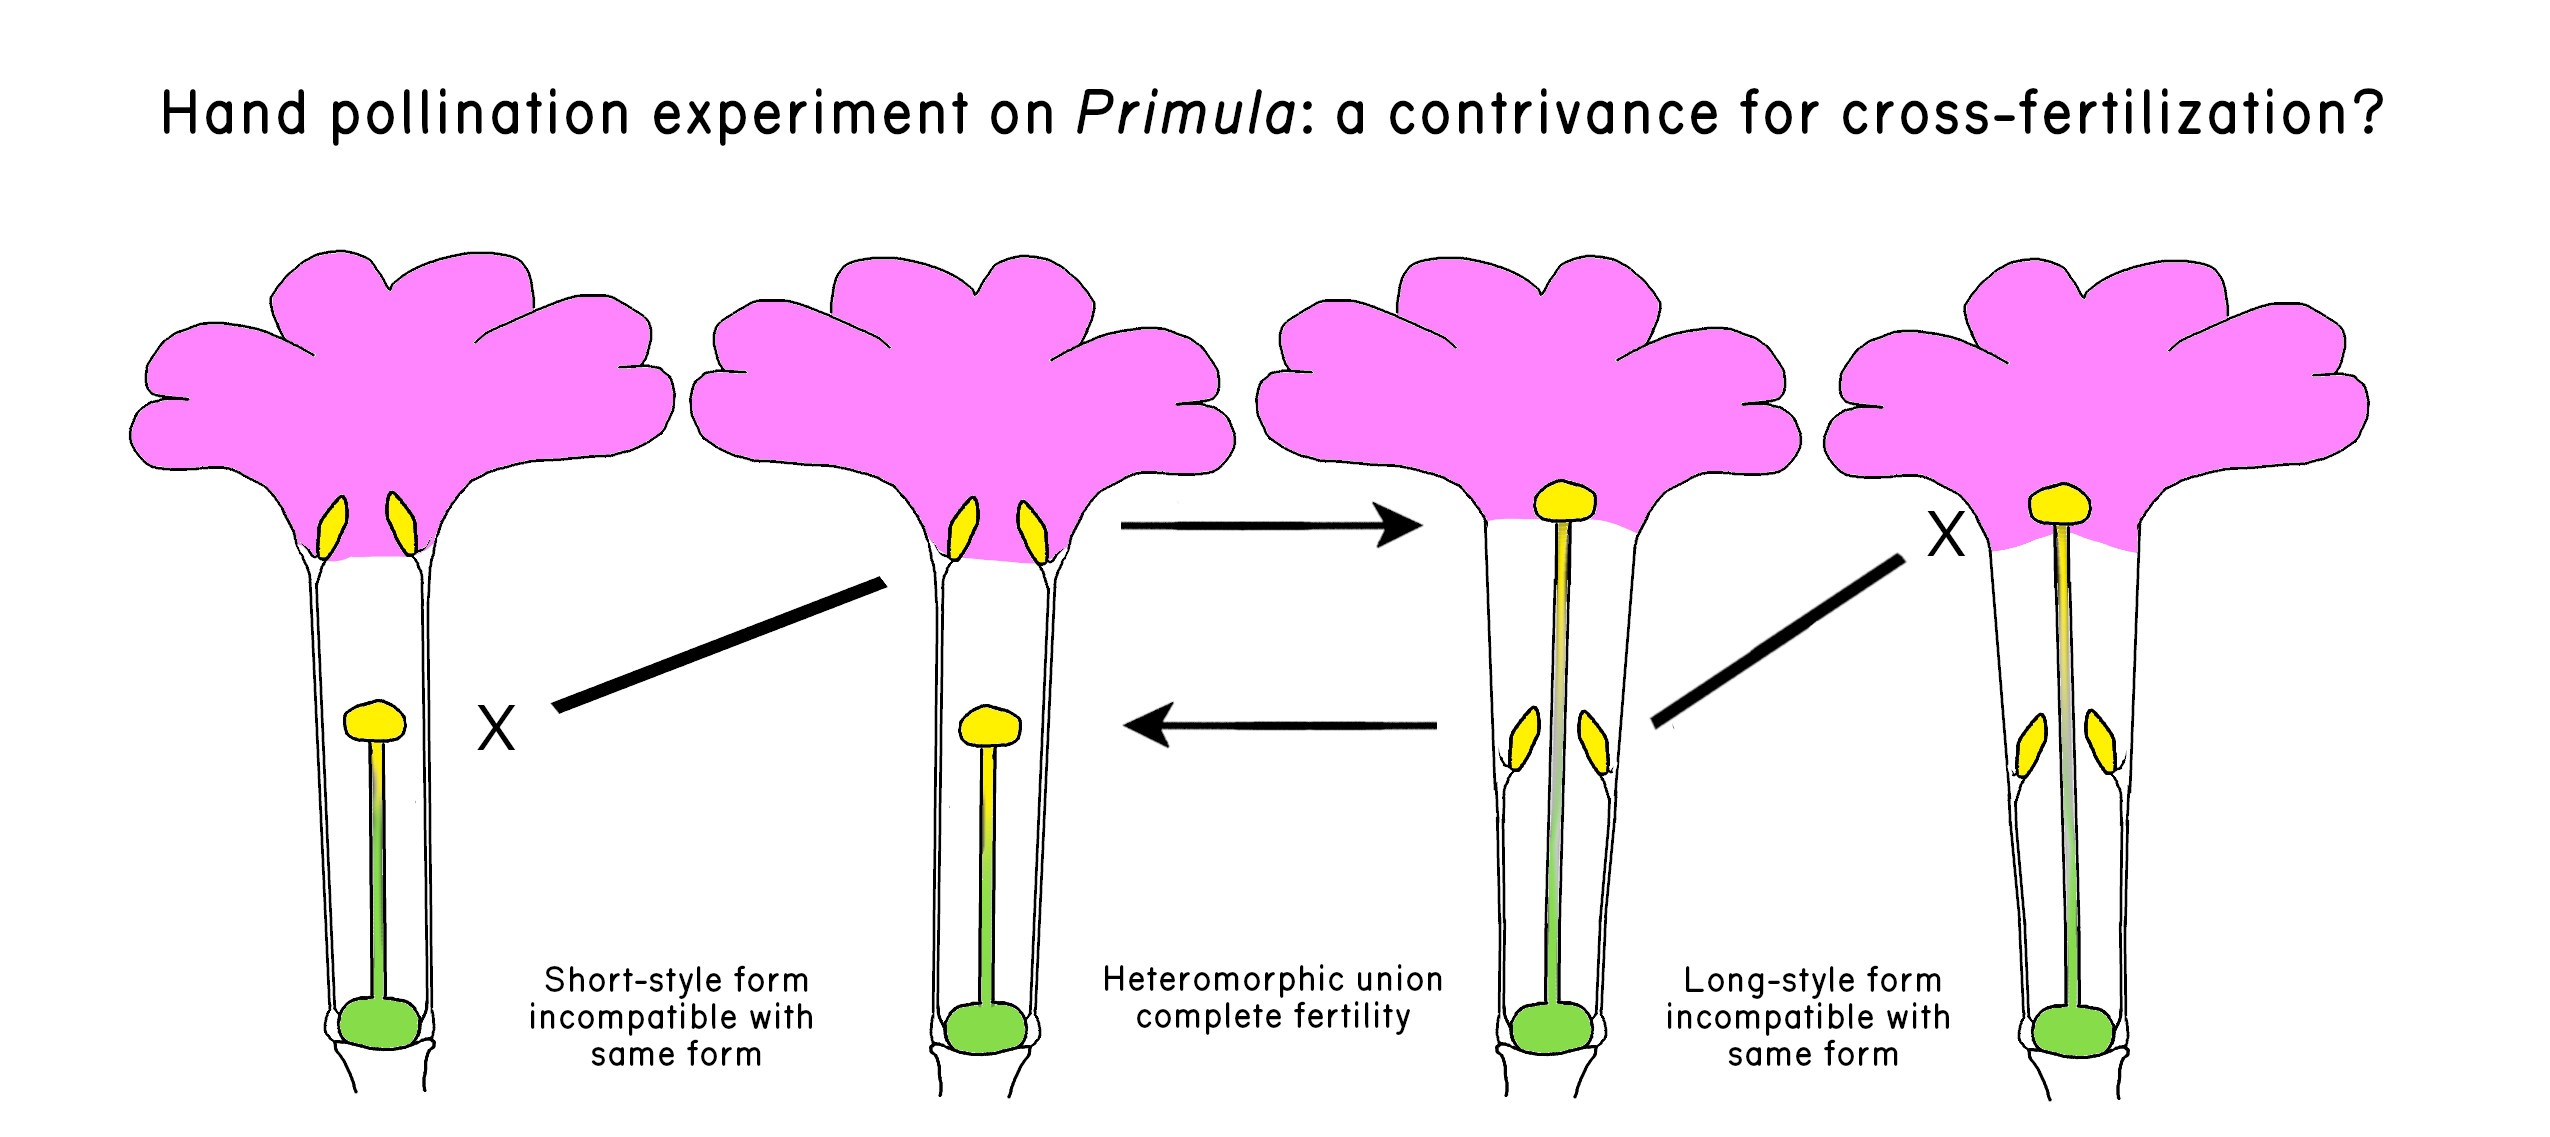
\includegraphics[width=1.25\textwidth,height=\textheight]{images/fig1-3.jpg}

}

\end{figure}

\hypertarget{darwins-view}{%
\subsection{Darwin's view}\label{darwins-view}}

Even before the cost of males and meiosis were so dramatically revealed
by Williams and Maynard Smith, biologists were reckoning with the
anomaly of sex (reviews in Meirmans 2009, Dagg 2016). One of the
earliest of these biologists was Charles Darwin. After he published the
\emph{Origin of Species}, Darwin was doing hand-pollination experiments
at Down House on three species of a curious annual plant in the genus
\emph{Primula}. The plant is curious in that it has two morphs. One
morph has a style that extends beyond the anthers (the long-style
morph), and the other morph has anthers that extend beyond the style
(the short-style morph). Botanists refer to this condition as distyly
(Figure~\ref{fig-1.3}). Darwin found that crosses between the different
morphs of the same species resulted in a very successful production of
seeds, but crosses between unrelated individuals of the same morph were
dramatically less successful (Darwin 1862). In discussing these results,
Darwin speculated that the two morphs may have evolved to insure
cross-fertilization: ``Whether or not the dimorphic condition of the
\emph{Primula} has any bearing on other points in natural history, it is
valuable as showing how nature strives, if I may so express myself, to
favour the sexual union of distinct individuals of the same species.''''

Darwin then asks a killer question. Why should the union of elements
from distinct individuals be favored? Why, in fact, is there sex? ``Nor
do we know why nature should thus strive after the intercrossing of
distinct individuals. We do not even in the least know the final cause
of sexuality; why new beings should be produced by the union of the two
sexual elements, instead of by a process of parthenogenesis. The whole
subject is as yet hidden in darkness.'' Darwin's question shows that the
cross-fertilization is curious, even without considering the costs of
sex. It also shows how Darwin was drawn to anomalies on
theory\footnote{We were trained ask questions first and then seek
  suitable organisms to address the questions. This was the tradition
  before model-systems research took over (Churchill 1997).}.

It is interesting to note that, in Darwin's quote above, he switches
from discussing mechanisms to prevent self-fertilization, such as
distyly, to discussing parthenogenesis. Self-fertilization is a sexual
process (involving the formation and fusion of gametes from the same
parent), while parthenogenesis is an asexual process that does not
generally involve meiosis and syngamy (review in Bell 1982). But
parthenogenesis and self-fertilization are conceptually related, as they
are both uniparental forms of reproduction. Hence, it makes sense that
Darwin would switch back and forth between these two different forms of
uniparental reproduction. Why cross-fertilize if either selfing or
parthenogenesis is an option?

There may be another reason why Darwin pivots to parthenogenesis. Just
prior to the publication of Darwin's (1862) paper on \emph{Primula},
Carl Theodor Ernst von Siebold (1856) published his observations on the
successful development of adults from unfertilized eggs, which he called
``parthenogenesis'' (virgin birth). These were revolutionary
observations, which caught Darwin's attention. In a letter to his
mentor, J.S. Henslow, Darwin mentioned von Siebold's discovery as
follows: \emph{There is no greater mystery in the whole world, as it
seems to me, than the existence of sexes, -- more especially since the
discovery of Parthenogenesis}. Letter to J. S. Henslow. See
\href{https://www.darwinproject.ac.uk/letter/DCP-LETT-2869.xml}{Darwin
Correspondence Project}.

However, the discovery of parthenogenesis\footnote{Prof.~Winterbourn was
  supportive of my work from this first day. He shared his knowledge of
  the snail system and of freshwater ecology, in general, with great
  enthusiasm. In addition, Mike met with my Ph.D.~students and took them
  into the field. This book would not have been possible without
  Prof.~Winterbourn.} was met with some hostility. Consider, for
example, the following statement by Rudolf Wagner in his 1857 review of
von Siebold's book on parthenogenesis {[}as translated from the original
German by Churchill (1979){]}: ``I must unfortunately say that one of
the most unpleasant of facts, {[}\emph{Parthenogenesis}{]} has been
introduced into physiology, which for the hope of so-called general laws
of animal life-phenomena \emph{is most distasteful}. It is impossible,
considering the glorification of our highly vaunted progress in the
theoretical understanding of the life processes, for it to be welcomed
or particularly encouraged; and sincerely speaking, I can be as little
pleased about it as a physicist would be if suddenly one or more
exceptions to the law of gravitation were discovered'' (Emphasis added).

Clearly, Wagner was not pleased with the discovery of asexual
reproduction, calling it unpleasant, unwelcome, and distasteful. By
contrast, Darwin did not find the idea to be distasteful in any way. He
wondered instead why it was not more common. For example, Darwin (1868)
wrote: \emph{Parthenogenesis is no longer wonderful; in fact, the wonder
is that it should not oftener occur}.\footnote{See also Elliott and
  Brook (2007). They point out crucial differences between Chamberlin
  and Platt including that Chamberlin allowed for multiple ideas to be
  partially correct, which is important for Chapter~\ref{sec-chap6}.}

Over 100 years later, W. D. Hamilton (1975) was also pondering the
evolution of outcrossing, and he wrote something conceptually similar:
``\ldots complete inbreeding abandons the obviously important advantages
of sexual reproduction, whatever these are.''''

Whatever these are! The advantages of outcrossing were obviously
important because cross-fertilization is so dominant. But the source of
these advantages was not clear. At about the same time, Maynard Smith
(1976) mused: ``One gets the feeling that some essential feature of the
situation has been overlooked.''

I now think that John Maynard Smith was correct. An essential feature
had indeed been overlooked: parasites.

\hypertarget{summary}{%
\section{Summary}\label{summary}}

\begin{enumerate}
\def\labelenumi{\arabic{enumi}.}
\tightlist
\item
  Obligate sexual reproduction is subject to invasion and replacement by
  all-female asexual lineages that do not pay the cost of males.
\item
  Obligate outcrossing in simultaneous hermaphrodites is subject to
  invasion and replacement by self-fertilization unless inbreeding
  depression is severe.
\item
  The exchange of DNA between different parental chromosomes
  (recombination) is similarly paradoxical.
\item
  Why then are recombination and cross-fertilization so common?
\end{enumerate}

\begin{tcolorbox}[enhanced jigsaw, left=2mm, bottomtitle=1mm, opacitybacktitle=0.6, breakable, leftrule=.75mm, coltitle=black, titlerule=0mm, opacityback=0, arc=.35mm, colback=white, title=\textcolor{quarto-callout-note-color}{\faInfo}\hspace{0.5em}{Box 1.2}, toprule=.15mm, rightrule=.15mm, bottomrule=.15mm, colframe=quarto-callout-note-color-frame, toptitle=1mm, colbacktitle=quarto-callout-note-color!10!white]

Maynard Smith's (1978) model showing the cost of producing
males.\footnotemark{} Let \(N_{asex}\) be the number of asexual females
at time 1, while \(N_{sex}\) gives the total number of sexual
individuals (males plus females) at time 1. Let \(B_{asex}\) give the
number of offspring produced by asexual females, and \(S_{asex}\) gives
the survival probability of asexual offspring to maturity. The number of
surviving asexual offspring is then \(= B_{asex}S_{asex}\). Similarly,
let \(B_{sex}\) be the number offspring produced by sexual females, and
let \(S_{sex}\) give the survival probability of sexually produced
offspring. Maynard Smith assumed that all individuals reproduce once and
then die. Let \(r\) be the frequency of females in the sexual
population. The number of asexuals and sexuals at time 2 can then be
calculated as is the table below. (Note, we do not assume that the
population is at carrying capacity).

\begin{longtable}[]{@{}
  >{\centering\arraybackslash}p{(\columnwidth - 4\tabcolsep) * \real{0.1607}}
  >{\centering\arraybackslash}p{(\columnwidth - 4\tabcolsep) * \real{0.2262}}
  >{\centering\arraybackslash}p{(\columnwidth - 4\tabcolsep) * \real{0.6131}}@{}}
\toprule\noalign{}
\begin{minipage}[b]{\linewidth}\centering
\end{minipage} & \begin{minipage}[b]{\linewidth}\centering
\textbf{Time 1}
\end{minipage} & \begin{minipage}[b]{\linewidth}\centering
\textbf{Time 2}
\end{minipage} \\
\midrule\noalign{}
\endhead
\bottomrule\noalign{}
\endlastfoot
\textbf{N. of asexuals} & \(N_{asex}\) &
\(N_{asex}(S_{asex}B_{asex})\) \\
\textbf{N. of sexuals} & \(N_{sex}\) & \(rN_{sex}(S_{sex}B_{sex})\) \\
\textbf{Freq. of asexuals} & \(\frac{N_{asex}}{N_{asex} + N_{sex}}\) &
\(\frac{N_{asex}(S_{asex}B_{asex})}{N_{asex}(S_{asex}B_{asex})+rN_{sex}(S_{sex}B_{sex})}\) \\
\end{longtable}

The fold increase in frequency of asexuals, \(F\), is the ratio of the
frequency of asexuals at time 2 divided by the frequency of asexuals at
time 1 giving:

\[F = \frac{N_{asex}(S_{asex}B_{asex})}{N_{asex}(S_{asex}B_{asex}) + r(N_{sex}S_{sex}B_{sex})}/\frac{N_{asex}}{N_{asex} + N_{sex}}\]

Under the all-else-equal assumption, \(S_{asex} = S_{sex}\) and
\(B_{asex} = B_{sex}\), giving:

\[F = \frac{N_{asex}}{N_{asex} + rN_{sex}}/\frac{N_{asex}}{N_{asex} + N_{sex}}\]

Assuming that there is a single asexual female at time 1, we get

\[F = \frac{1}{1 + rN_{sex}}/\frac{1}{1 + N_{sex}} = \frac{1 + N_{sex}}{1 + rN_{sex}}\]

If \(N_{sex}\) is very large, the solution reduces to \(F \approx 1/r\).
Hence, the fold increase in the frequency of asexuals, \(F\), is
inversely related to the frequency of females \((r)\) in the sexual
subpopulation. Assuming a 1:1 sex ratio, \(r = 0.5\). Hence, for an
equal sex ratio, the increase in asexuals is \(\approx\) 2-fold. This
result gives the two-fold cost of males. Assuming ``all-else-equal'' a
clone will double when rare when introduced into a large sexual
population.

\end{tcolorbox}

\footnotetext{With respect to \emph{Potamopyrgus} (along with a
parthenogenetic beetle) Maynard Smith (1978, page 65) wrote, ``Further
Investigations of these cases could be most interesting.'' When I met
JMS, I did not know (or did not remember) that he had written this. But
I think that he was correct.}

\hypertarget{sec-eco-hyp}{%
\chapter{The Ecological Hypotheses}\label{sec-eco-hyp}}

\begin{figure}

{\centering 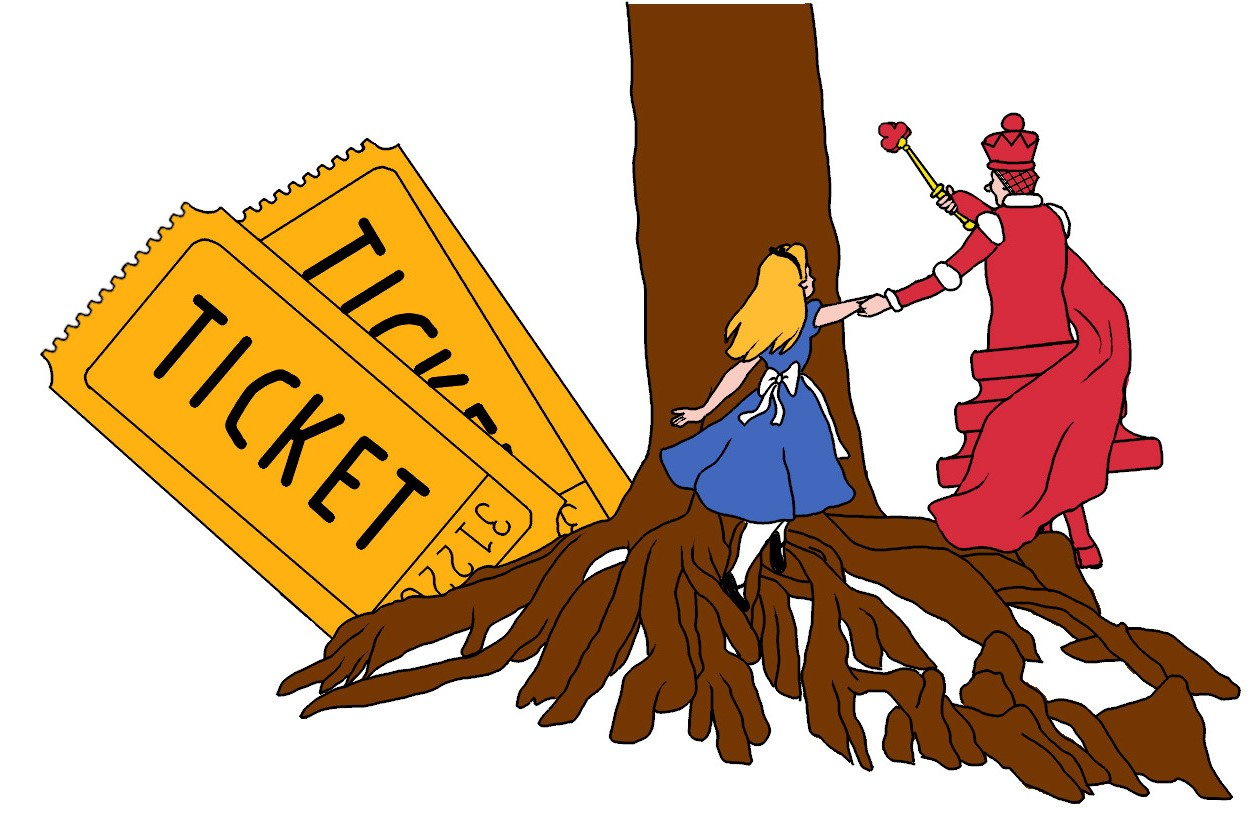
\includegraphics{images/fig2-1.jpeg}

}

\end{figure}

The sex/recombination (``sex/rec'') anomaly has attracted some of the
best theoretical biologists over the last 50 years, leading to at least
two dozen hypotheses to explain selection for recombination and/or the
persistence of obligate sexual reproduction in natural populations
(Kondrashov 1993). In what follows, I first focus on the ecological
hypotheses. The ideas underlying these hypotheses provide a handle for
understanding some of the foundational concepts in evolutionary ecology.

\hypertarget{the-lottery-model}{%
\section{The Lottery Model}\label{the-lottery-model}}

As part of his book on the evolution of sex, Williams (1975) suggested
that sex could be favored in fluctuating abiotic environments. The idea
is intuitive: cross-fertilization generates variation among offspring.
Hence, in fluctuating environments, sex could increase the probability
that some offspring might survive. Williams likened the idea to a unique
kind of lottery. For example, he wrote: ``Suppose you were offered this
choice in a lottery: either you could have several different tickets, or
you could have the same number of copies of the same ticket'' (p.~15).
If you choose \emph{N} copies of the same ticket (asex), and your ticket
wins, you get \emph{N} times the reward. If you choose \emph{N}
different tickets (sex), you increase the probability of winning
something, but the reward is smaller. Williams referred to the idea as
the aphid-rotifer model, but the idea has since come to be known as the
Lottery Model (following Bell 1982), which is a more descriptive
phrase.\footnote{I ran two years of field experiments designed to test
  for random settlement by genetically determined morphs. I also ran
  experiments designed to test for habitat selection by genetically
  determined morphs. The results were always negative. I finally tested
  for predator-induced development of the bent morph by placing
  \emph{Acanthina} snails in quadrats where juvenile barnacles had
  recently settled. I used herbivorous snails as a control. The results
  showed that the presence of \emph{Acanthina} induced development of
  the bent form, but the herbivorous snails did not. It was a thrilling
  discovery.}

In my evolution course, I ask a form of Williams' question, but with a
slight twist:

\begin{quote}
If you had a garden, upon which your descendants will depend for many
generations to come, would you

\begin{enumerate}
\def\labelenumi{\arabic{enumi}.}
\tightlist
\item
  plant a genetically variable crop, or
\item
  a monoculture with a two-fold higher yield?
\end{enumerate}

Keep in mind that your descendants will follow your choice.
\end{quote}

Often the students rightfully want some clarification. They ask, for
example, ``Can we use pesticides?'' But every time, most students choose
the variable crop. I remind them that selecting the variable crop will
reduce their yield by one half. They don't budge. I re-ask the question,
doubling the relative yield for the monoculture from two-fold to
four-fold. Then to 10-fold. Occasionally, one of the more risk-prone
students will select the 10-fold higher yield, but most do not budge.
They want genetic variation. I ask them why. Invariably, they say that
the environment is going to change. They want to hedge their bets
against an uncertain future.

Indeed, Williams' Lottery Model is about bet hedging. The gist of
bet-hedging in evolutionary theory is that selection can act to reduce
the variance in reproductive success over time, even if it also reduces
the arithmetic mean across years (review in Philippi and Seger 1989).
Suppose, for example, that we have the following data for both a
monoculture and a genetically variable polyculture (in arbitrary units).
Let's assume that the variation in yield is driven by annual variation
in abiotic factors, such as temperature or precipitation. The effect of
planting a polyculture (bet-hedging) can be estimated from the geometric
mean, which incorporates the variation in yield over time.

\begin{longtable}[]{@{}lll@{}}
\toprule\noalign{}
Year & Monoculture & Polyculture \\
\midrule\noalign{}
\endhead
\bottomrule\noalign{}
\endlastfoot
1 & 350 & 250 \\
2 & 400 & 250 \\
3 & 300 & 200 \\
4 & 100 & 200 \\
5 & 50 & 200 \\
& & \\
\textbf{Arithmetic mean} & \textbf{240} & 220 \\
\textbf{Variance}\footnote{Plasticity is more mainstream now than it was
  in the 1980s. One reviewer of my paper was incredulous and recommended
  rejection from \emph{Evolution} because the bent morph was not
  ``genetically determined.'' The Associate Editor (John Endler)
  rejected the review and accepted the paper. Clearly, it is the
  developmental strategy that is genetically determined, not the morph
  per se (see also Lively et al.~2000, Hazel et al.~2004).} & 19400 &
600 \\
\textbf{Geometric mean (GM)}\footnote{Facultative parthenogenesis is
  used to mean environmentally cued production of parthenogenetic
  females. I was originally planning to work on a nematode population
  that produced a mixture of sexual males and females at high density
  but only parthenogenetic females at low density.} & 184 &
\textbf{219} \\
\textbf{Approximate GM} & 200 & \textbf{219} \\
\end{longtable}

In this example, we find that the monoculture has an arithmetic mean of
240, while the polyculture has an arithmetic mean of only 220. So, I
might be inclined to plant the monoculture. However, the among-year
variance is very high for the monoculture (relative to the polyculture),
driven in large part by the low yields in years 4 and 5. By contrast,
the geometric mean for the monoculture is 184, while the geometric mean
for the polyculture is 219. Based on this, I might be inclined to plant
the polyculture, as it reduces the cost of very low yield in bad years.
I think the students see this intuitively. Over the long term, it is
better to be risk-averse and plant the genetically variable polyculture.
What if, for example, the monoculture produced no food in the last year?
The geometric mean would be zero. That would be catastrophic.

The effect of variance on the geometric mean (GM) can be seen by an
approximation (Stearns 2000):

\[\text{GM} \approx \overline{x} - \frac{\text{var}(x)}{2\overline{x}}\]

where \(\overline{x}\) is the mean, and var(\(x\)) is the variance in
\(x\). Note that the approximation is equal to the arithmetic mean when
the variance in \(x\) is zero. Note too that the geometric mean
increases as the variance in \(x\) decreases. So, if selection operates
to reduce the among-year variance in fitness, the outcome of selection
will be reflected by an increase in the geometric mean. In general,
evolutionary biologists use the geometric mean (rather than the
arithmetic mean) to measure fitness over time.\footnote{We were trained
  ask questions first and then seek suitable organisms to address the
  questions. This was the tradition before model-systems research took
  over (Churchill 1997).}

Can sex be favored in variable environments as a bet-hedging strategy?
It seems like a very sensible idea, provided that the production of
genetically variable progeny reduces the among-year variance in
offspring survival. But remember, that under a two-fold cost of sex,
asexuals can replace large populations of sexuals in tens of generations
(see chapter 1). So, if the Lottery Model is correct, significant
environmental change must occur very rapidly. The many thousands of
years between ice ages, for example, would be too long.

\hypertarget{the-tangled-bankfrozen-niche-variation-model}{%
\section{The Tangled Bank/Frozen Niche-Variation
Model}\label{the-tangled-bankfrozen-niche-variation-model}}

Roughly speaking, the Lottery Model concerns the value of producing
diverse offspring in a temporally variable abiotic environment. A
different kind of model instead concerns the role of competition for
different resource types that vary in space. Let us first consider the
Frozen Niche-Variation Hypothesis of Robert Vrijenhoek. The key idea is
that the clonal derivatives of sexual ancestors ``freeze'' some of the
genetic variation in the sexual population. This frozen genotype then
determines the resource niche of the clone. It seems reasonable to
assume that the niche width of a single clone would be relatively narrow
compared to the niche width of the genetically diverse sexual
population. So, under this idea, a clone could invade a sexual
population, and perhaps displace it from one of its many niches. But a
single clone could not completely replace the sexual population
(Vrijenhoek 1979). This kind of process could explain those situations
in which sexual and asexual females coexist, which was a major
advance.\footnote{Prof.~Winterbourn was supportive of my work from this
  first day. He shared his knowledge of the snail system and of
  freshwater ecology, in general, with great enthusiasm. In addition,
  Mike met with my Ph.D.~students and took them into the field. This
  book would not have been possible without Prof.~Winterbourn.}

A conceptually similar model was independently developed by Graham Bell:
the Tangled Bank Hypothesis (Bell 1982). Bell nabbed the name from the
last paragraph of the \emph{Origin of Species}, in which Darwin imagines
life as an ``entangled bank'' of species interacting in a complex
network. The core of the idea can be traced back to Howard Levene's
(1953) pioneering model, which showed that polymorphism could be
maintained in a spatially heterogeneous environment provided that
different genotypes specialize on different resources. Levene's model
was a major advance, as it showed that genetic diversity could be
maintained without heterozygote advantage
(\protect\hyperlink{callout-2.1}{Box 2.1}). This was also one of the
first models to fuse population genetics with ecology. But how does
multiple niche polymorphism apply to sex? The idea is that, if selection
results in polymorphism, then a genetically diverse sexual population
might be resistant to replacement by a clonal lineage that specializes
on only one of the available resource types (as also in the Frozen
Niche-Variation Model).

Here is how I pose the Tangled Bank idea to my undergraduate students. I
start by giving them a choice between two hypothetical resources, which
occur in different parts of the room. One is pizza, the other is
broccoli. They all choose pizza. The problem, of course, is that the
per-person value of the pizza resource declines as the pizza-eating
population grows. At some point, there will be an advantage to
specializing on broccoli. This could lead to a polymorphic population
composed of obligate pizza eaters and obligate broccoli eaters, where
(at equilibrium) the value of both resources is the same. Hence,
selection for or against a particular strategy depends on the frequency
of that strategy in the population. Perhaps this kind of
\emph{frequency-dependent selection} could favor sexual reproduction as
a way to diversify offspring in environments where different resource
types are patchily distributed in space. This reasoning forms the
essence of the Tangled Bank Hypothesis.

One especially interesting aspect of the Tangled Bank Model is that the
strength of frequency-dependent selection depends on population density.
For example, there would be no selection to utilize the resource of
lower value (broccoli) if there were no competition for pizza. This kind
of selection, where the advantage to being rare depends on population
density, is sometimes referred to as ``soft'' selection (Wallace
1975).\footnote{See also Elliott and Brook (2007). They point out
  crucial differences between Chamberlin and Platt including that
  Chamberlin allowed for multiple ideas to be partially correct, which
  is important for Chapter~\ref{sec-chap6}.} In other words, soft
selection is selection that is both frequency-dependent and
density-dependent. This idea contrasts nicely with the Lottery Model,
where selection is both frequency- and density-independent, which is
called ``hard'' selection. For our purposes, we can use Wallace's
terminology to conceptually separate the Tangled Bank Hypothesis from
the Lottery Model Figure~\ref{fig-2-2}.

\begin{figure}

\sidecaption{\label{fig-2-2}Partitioning the ecological hypotheses for
the maintenance of obligate sexual reproduction. The figure is redrawn
from Wallace (1975). The inserted blue text shows how the ecological
hypotheses fit into Wallace's matrix for density-dependent selection vs
frequency-dependent selection. The Lottery Model relies on hard
selection in temporally variable environments. The Tangled Bank relies
on soft selection in spatially variable environments. The Red Queen
relies on frequency-dependent selection generated by coevolving
antagonistic species.}

{\centering 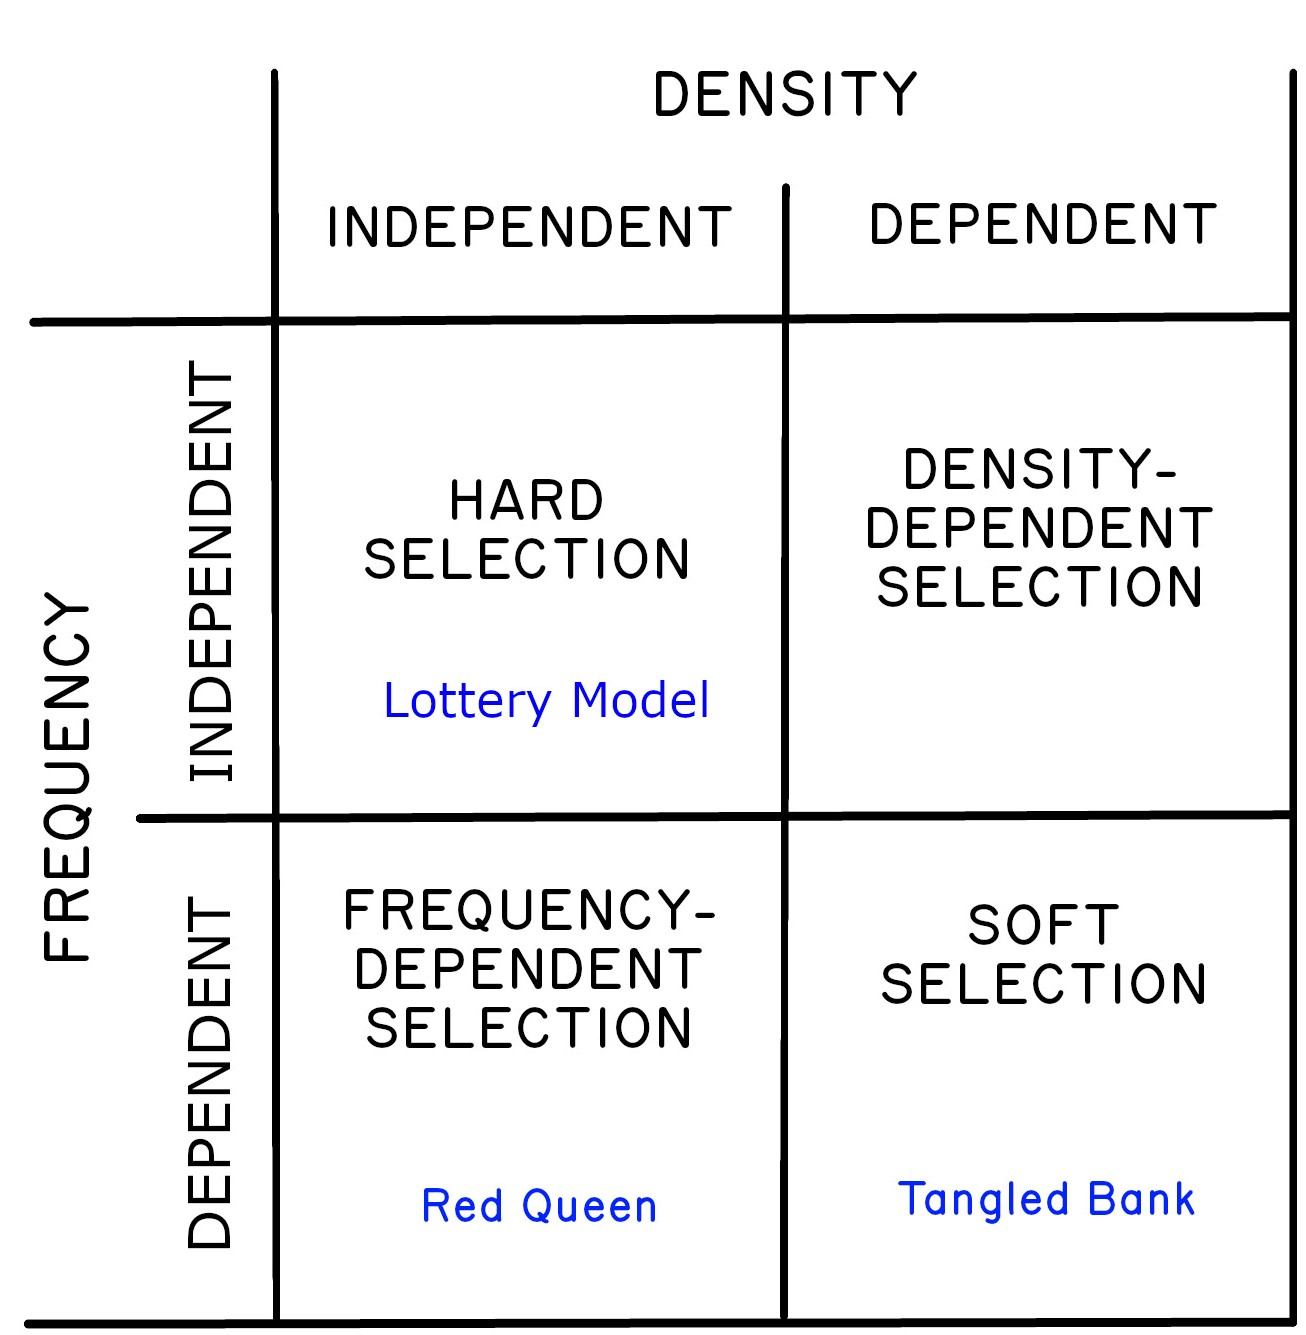
\includegraphics[width=0.75\textwidth,height=\textheight]{images/fig2-2.jpeg}

}

\end{figure}

We can think of the contrast like this. Under the Lottery Model, changes
in the environment will select against certain genotypes independent of
whether they are common or rare. Selection seems unconditional (hard).
Under the Tangled Bank, selection is always conditional (soft); there is
an advantage to having a rare genotype, but this advantage only accrues
under strong competition (high density). Soft selection may not be
exactly the best possible phrase, but it contrasts nicely with hard
selection.\footnote{With respect to \emph{Potamopyrgus} (along with a
  parthenogenetic beetle) Maynard Smith (1978, page 65) wrote, ``Further
  Investigations of these cases could be most interesting.'' When I met
  JMS, I did not know (or did not remember) that he had written this.
  But I think that he was correct.}

Two caveats are worth mentioning with respect to soft selection and the
Tangled Bank Hypothesis. One is that polymorphism is only stable under a
narrow range of patch-types frequencies. In addition, strong tradeoffs
are required for the cost and benefits for morphs occupying different
patches (Maynard Smith and Hoekstra 1980, Lively 1986a) (see also
\href{https://iulibscholcomm.github.io/through-the-looking-glass/eco-hyp.html\#callout-4}{Box
3.1}). The second caveat is that repeated mutation to asexual
reproduction could lead to the accumulation of clonal diversity over
time. Once all the niches are occupied by different specialized clones,
there would be no advantage to sex. A diverse clonal population could
then replace the sexual population (Bell 1982, Vrijenhoek and Parker
2009). This second caveat applies, in general, to any model of sex that
relies on frequency-dependent selection. But the ideas could work if
mutations to asex are rare. And, as I mentioned, sexuals and asexuals
are known to coexist in some populations, which is consistent with the
Tangled Bank and Frozen Niche-Variation Hypotheses (Vrijenhoek and
Parker 2009). Coexistence, however, is also compatible with the Red
Queen hypothesis, which we will now consider.

\hypertarget{the-red-queen-hypothesis}{%
\section{The Red Queen Hypothesis}\label{the-red-queen-hypothesis}}

The Red Queen Hypothesis is like the Lottery Model in that it focusses
on environmental change over time. However, under the Red Queen idea,
the change is mediated by changes in coevolving biological antagonists
such as parasites, rather than changes in the abiotic
environments.\footnote{This assumption turned out to be not strictly
  true. Polyploid females occasionally produce males, although they seem
  unlikely to be very fertile (Soper et al.~2013).} The distinction is
important, as we will see.

It may be helpful to revisit Figure~\ref{fig-1-2}, which shows the
replacement of a sexual population by a clonal lineage within 25
generations. In this example, the clone was a single genotype, while the
sexual population was composed of multiple recombining genotypes, only
one of which was shared with the clone. Clearly, as the clone spreads,
its genotype would become the most common in the host population. Now
suppose that the host population is coevolving with a parasite
population, which is composed of multiple strains. Assuming random
contact between hosts and parasites, the parasite strain that could
infect the most common host genotype would have a selective advantage
over parasite strains that could only infect rare host genotypes. Let's
call this more successful parasite strain ``strain \textbf{A}.'' What
would happen? It should be easy to see that strain \textbf{A} would
increase in frequency. The parasite population would evolve.

Now, what if the parasite dramatically reduces the reproductive success
of infected hosts? We might expect that, as the parasite evolves to
infect the most-common host genotype, the reproductive advantage of the
host clone is eroded. Moreover, if the parasite is \emph{common and
sufficiently virulent}, evolution by the parasite could prevent the
clone from eliminating the sexual population. Under this scenario, there
are at least two possible outcomes. One is that the sexuals and asexuals
come to exist in stable frequencies, where the lost fecundity of the
clone due to infection is equal to the cost of males, meaning that the
mean fitnesses of sexuals and asexuals are equal. On the other hand, if
the parasite is highly virulent, the frequencies of sexuals and asexuals
can oscillate over time (Figure~\ref{fig-2-3} A). Under this second
scenario, the new clone initially increases, but it is driven down
sharply by infection (Figure~\ref{fig-2-3} B). Then, once the clone
becomes very rare, it should become less infected than observed in the
sexual population (Figure~\ref{fig-2-3} B). During this period, there is
parasite-mediated selection against sex. Hence, the clone increases in
frequency (Figure~\ref{fig-2-3} A), only to be driven down again by
parasites after it becomes common (Figure~\ref{fig-2-3} B). Another
cycle begins. \textbf{The key point is that parasites do not select
against clonal reproduction per se; they only select against common
genotypes.} But selection against common host genotypes might be
sufficient to prevent fixation of a clone in the short term.

\begin{figure}

\sidecaption{\label{fig-2-3}Simulation model showing that coevolving
parasites can prevent the fixation of asexuals in the short term.
\textbf{A.} The number of sexual and asexual individuals over time.
\textbf{B.} The frequency of infection in sexual and asexual individuals
over time. The simulation introduces a single clonal genotype into a
sexual population at carrying capacity. After the clone becomes common
(\textbf{A}) the parasites evolve to ``target'' it for infection
(\textbf{B}). Note that after the parasites have driven the clone's
frequency down, the asexuals are less infected than the sexuals.
Simulation model based on Lively (2009), which treats parasite virulence
as a positive function of host density.}

{\centering 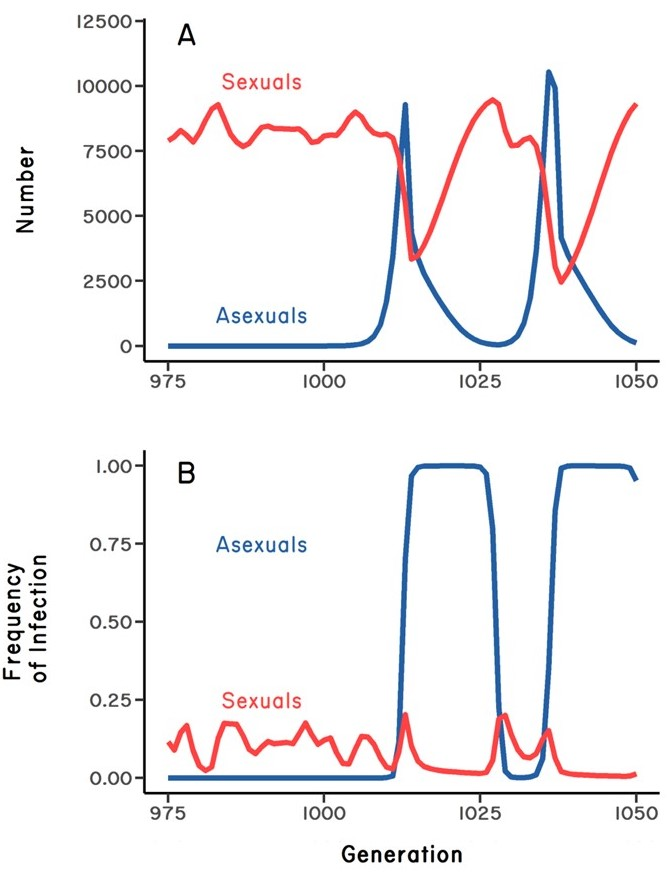
\includegraphics{images/fig2-3.jpg}

}

\end{figure}

This scenario of fluctuating selection for and against sex is just a
special case of the more general idea that parasites will select against
common genotypes within a diverse, sexual host population. As a rare
host genotype becomes common, the parasites genotype that can infect it
will be favored by natural selection. If the parasite is virulent
(meaning that infection reduces host fitness), the targeted host
genotype will decline in frequency, and a new host genotype will begin
to increase in frequency. Under this logic, host-parasite coevolution
will lead to the oscillation of genotypes in both the host and the
parasite populations (Figure~\ref{fig-2-4}). These oscillations are now
called Red Queen dynamics. Red Queen dynamics can lead to the
maintenance of genetic polymorphism in sexual populations, and possibly
protect sexual reproduction from replacement by asexual lineages. In
addition, Red Queen dynamics could also favor recombination within a
sexual population (Peters and Lively 1999, Schmid-Hempel and Jokela
2002, Peters and Lively 2007, Salathe et al.~2008). These related ideas
are now called the Red Queen Hypothesis (following Bell 1982).

\begin{figure}

\sidecaption{\label{fig-2-4}Red Queen dynamics. The frequency of a
single host genotype is shown along with the frequency of the only
parasite genotype that can infect it. Note that the parasite tracks the
host with a time lag. Results were extracted from a simulation of a
sexual host population with nine possible genotypes coevolving with an
asexual parasite with nine matching genotypes Lively (2009). The dashed
line shows the average genotype frequency for hosts and parasites.}

{\centering 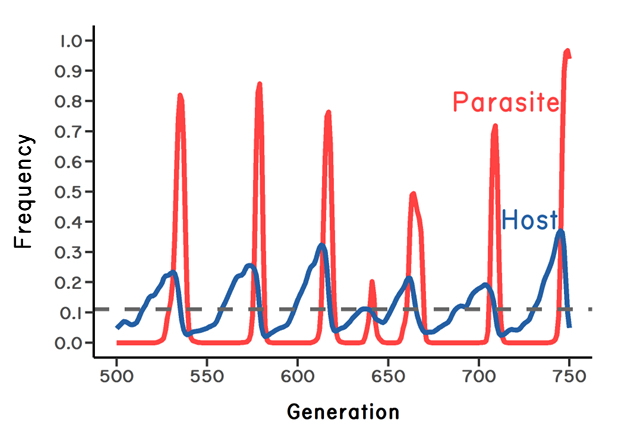
\includegraphics{images/fig2-4.jpeg}

}

\end{figure}

\hypertarget{an-intersection-of-science-and-literature}{%
\subsection{An intersection of science and
literature}\label{an-intersection-of-science-and-literature}}

The name for the Red Queen Hypothesis comes from \emph{Through the
Looking Glass} (Carroll 1872). Here are the relevant bits of the story.
After Alice goes through the looking glass (a mirror), she decides to
follow a straight path to the top of a hill. But, in following the path,
she ends up at her starting point. Talking to herself, she remarks,
``But how curiously it twists! It's more like a corkscrew than a path.''
Repeated attempts were unsuccessful. In frustration, Alice addresses a
tiger lily amongst a patch of flowers, ``I wish you could talk!'' The
lily informs Alice that all the flowers can talk. The stunned Alice then
begins a conversation with the flowers before finally asking, \emph{Are
there more people in the garden besides me?} The rose answers \emph{yes,
there is someone like you.} Alice sets out to follow this person (the
Red Queen), but she quickly loses sight of her, and ends up back at her
original starting point. Flustered, Alice decides to follow the advice
of the rose: ``I should advise you to walk the other way.'' Alice then
quickly finds the Red Queen.

Now it gets especially interesting. Alice mentions to the Red Queen that
she would like to ``find my way to the top of the hill.'' The Red Queen
replies: ``I could show you hills in comparison with which you'd call
that a valley.'' Alice protests: ``a hill ca'n't be a valley\ldots{}
That would be nonsense.'' This exchange between Alice and the Red Queen
now seems prophetic, because, under frequency-dependent selection,
locations on the adaptive landscape can rapidly change from fitness
peaks to fitness valleys. Perhaps the Red Queen's statement is correct:
hills can become valleys, and valleys can become hills. More
specifically, genotypes that were favored by natural selection when rare
can become selected against after they become common, leading to a
highly dynamic adaptive landscape.

In any case, Alice had clearly entered a crazy world. Straight paths
become like corkscrews, progress is made by going the other way, and
hills become valleys. Then, suddenly, Alice and the Red Queen began to
run: ``Alice never could quite make out, in thinking afterwards, how it
was that they began: all she remembers is, that they were running hand
in hand, and the Queen went so fast that it was all she could do to keep
up with her.'' During this furious run, Alice notices that they never
pass anything. The trees remain in the same place as if they were moving
along with them. Alice eventually asks: ``Are we nearly there?'' The Red
Queen replies: ``Why, we passed it ten minutes ago! Faster!''

When they finally stop, Alice is surprised to be where they started: ``I
do believe we have been under this tree the whole time! Everything is
just as it was!'' The Red Queen replies that of course, and then asks:
``What would you have it?'' Alice replies that she would have expected
to get somewhere else after running for a long time. The Red Queen then
replies with this very famous quote: ``Now, \emph{here}, you see, it
takes all the running \emph{you} can do to keep in the same place.'' It
is a perfect metaphor for host-parasite coevolution\footnote{The group
  included Mark McKone. Mark was a post-doc with David, and his comments
  were especially influential. Fifteen years later, I would become
  Ph.D.~advisor to one of Mark's star mentees at Carleton College,
  Maurine Neiman.}. Host and parasite genotypes might oscillate as if
they were running to stay in the same place.

It seems unlikely that Lewis Carroll had coevolution in mind when
writing these passages. But he was a mathematician at Oxford University
(his given name was Charles Dodgson), and at least one author has shown
how his writings can be seen as metaphors for mathematical problems
(Bayley 2009, 2010). Along these lines, mathematician Sanderson M. Smith
has suggested that
\href{http://www.herkimershideaway.org/writings/carroll.htm}{Carroll
simply inverted the equation for speed from ``speed = distance/time'' to
``speed = time/distance''}. Upon rearrangement, the latter gives
``distance = time/speed.'' Hence you must run very fast to stay in the
same place. But how does the shifting landscape fit in? And why did
Alice have to go the other way to meet the Red Queen? I would love to
know.

It is perhaps worth pointing out that the phrase ``Red Queen
Hypothesis'' can have two different meanings to evolutionary biologists.
In the early 1970s, Leigh van Valen was grappling with data showing that
the probability of extinction in very different organisms was
independent of the age of the lineage. He reasoned that, in
coevolutionary interactions, the probability of one species driving the
other species extinct could, in fact, be independent of lineage age (Van
Valen 1973). It thus seems reasonable to suggest that both antagonists
must run (coevolve) as fast as they can to prevent extinction. Graham
Bell repurposed the phrase to mean within-population oscillations in
host and parasite genotypes (Bell 1982). Hence, Van Valen's idea is
about macroevolution (speciation/extinction), while Bell's idea is about
microevolution. Even though van Valen's use of the Red Queen metaphor
was published first, I will use Bell's microevolutionary meaning, as it
perfectly captures the oscillating nature of genotype frequencies during
host-parasite coevolution.\footnote{There we also some very interesting
  outliers. Domesticated mammals had very strong positive residuals for
  the rate of recombination. This result suggests that recombination was
  selected by frequent changes in the targets of artificial selection by
  humans.}

\hypertarget{conceptual-roots-of-the-red-queen-hypothesis}{%
\subsection{Conceptual roots of the Red Queen
Hypothesis}\label{conceptual-roots-of-the-red-queen-hypothesis}}

Part of my goal is to show science as a process. As such it seems
reasonable to discuss the origins of the Red Queen idea. One of the
earliest statements alluding to the Red Queen Hypothesis came from W.D.
Hamilton (1975). Hamilton was reviewing the books by Williams (1975) and
Ghiselin (1974) for the \emph{Quarterly Review of Biology}. Throughout
the review, the reader can feel Hamilton's frustration with their
arguments. Towards the end, he makes this very abstract suggestion:
``\ldots it seems to me that we need environmental fluctuations around a
trend line of change'' and ``For the source of these we may look to
fluctuations and periodicities \ldots{} generated by life itself.''

The quote does not specifically refer to parasites, but it does suggest
that coevolutionary interactions, in general, could play a role in
selecting for sex and recombination. In his memoirs, Hamilton clears
this up, writing: ``At that stage when I wrote the review, although I
had not seen the particular relevance that parasitism might have, I had
for many years seen sex looming ahead and had reached a stage of being
excited by the possible primary role of biotic interaction. I had
decided that it was in aspects of the interspecies struggle, and not
survival in an inanimate environment, that I had to search for the main
factor. Adaptation to new physical habitats might be made possible
through sexuality but these adaptations could not be the main reason for
its existence (Hamilton 2001).''

Note that, here, Hamilton is specifically contrasting host-parasite
coevolution with the Lottery Model, which relies on random changes in
``physical habitats.''

At about the same time, a plant population biologist, Don Levin, was
also writing on the paradox of sex/rec. In his paper, Levin specifically
identified pathogens as a possible force selecting for recombination
(Levin 1975): ``I propose that the persistent tracking of plant hosts by
multiple pathogens and herbivores is a prime factor which prohibits the
congealing of the genomes of species, especially those in closed
communities.''

Boom! By ``prohibit the congealing of genomes,'' Levin means, ``selects
for recombination.'' The reference to ``closed communities'' means
species that are tightly coevolving in the absence of homogenizing gene
flow. This quote seems to be the first to specifically identify
coevolving pathogens as a primary source of selection favoring the
mixing of genomes. Levin's idea was quickly followed by important
conceptual contributions by Glesener \& Tilman (1978)\footnote{\begin{quote}
  Therefore, we attempt to treat the same problem with several
  alternative models each with different simplifications but with a
  common biological assumption. Then, if these models, despite their
  different assumptions, lead to similar results we have what we can
  call a robust theorem which is relatively free of the details of the
  model. Hence our truth is the intersection of independent lies (Levins
  1966).
  \end{quote}}, Jaenike (1978)\footnote{I was also persuaded by elegant
  experimental studies on sweet vernal grass, which showed a
  density-independent advantage to having a rare genotype (Antonovics
  and Ellstrand 1984, Ellstrand and Antonovics 1985). Later studies
  showed that the rare advantage was likely due to escape from infection
  (Kelley et al.~1988, Kelley 1993, 1994).}, and Lloyd (1980). In
particular, Lloyd writes: ``\ldots{} biological interactions are more
likely than unpredictable physical conditions to provide the kind of
relentless, repetitive change that is necessary for sexual parents to be
selected because of the genetic diversity that sex engenders.''

Lloyd then turns this abstract idea into a specific prediction, which I
would later test: ``If this proves to be so, we will then be able to
examine whether the occurrence of asexual reproduction is correlated
with relaxation of the biological hostility of the environment.'' Notice
that, in the quotes presented above, both Hamilton and Lloyd were
specifically predicting that coevolution is more important in selecting
for sex than uncertain physical environments. But it is reasonable to
ask, does it really matter? Aren't both ideas fundamentally about bet
hedging in uncertain environments? Yes: I think both ideas are about bet
hedging. But the distinction still matters. The Lottery Model is about
random shifts in the direction of selection; there is no selection
against common genotypes unless the environment changes by chance in a
way that disfavors them. By contrast, under the Red Queen, selection is
frequency dependent. In fact, selection against common genotypes is the
core of the model. Hence, the critical difference between the models is
not so much about bet hedging but whether selection for sex/rec is
directional (but randomly changing directions, a lottery) or frequency
dependent (Red Queen). For example, parasites could be a source of
directional selection for sex if they randomly changed which host
genotypes they attacked. To my mind, that would be a Lottery Model. The
Red Queen Hypothesis requires frequency-dependent selection generated by
interactions between species.\footnote{The partial correlation between
  percent male and prevalence of infection, while controlling for
  habitat, is highly significant (\(r = 0.36\), \(P < 0.001\)). However,
  the partial correlation between percent male and habitat, while
  controlling for prevalence of infection, is marginally significant
  (\(r = 0.21\), \(P = 0.05\)). Similar results were gained after males
  were excluded from the calculation of infection prevalence, which
  controls for any sex-specific differences in susceptibility (as shown
  in Figure~\ref{fig-3-4}); specifically, prevalence of infection in
  females was significantly correlated with male frequency while
  controlling for habitat (\(r = 0.37\), \(P < 0.001\)), but the
  converse was not true (\(r = 0.19\), \(P = 0.06\)).} This is an
important distinction.

Taking this view, the Red Queen Hypothesis may seem more closely related
to the Tangled Bank model than to the Lottery Model, as both the Red
Queen and the Tangled Bank rely on frequency-dependent selection. But
the critical distinction here is that selection against common genotypes
under the Tangled Bank relies on intraspecific competition in
populations at carrying capacity (soft selection). The Red Queen relies
on interspecific antagonistic coevolution, leading to parasite-mediated
selection against common host genotypes.\footnote{Using computer
  simulations, we recently found that detecting a significant positive
  correlation between clonal diversity and infection prevalence would
  only be expected in a fraction of parameter space, even when parasites
  were solely responsible for the maintenance of diversity (Lively et
  al.~2021).}

In any case, looking back, it seems clear that the architects of the
ecological hypotheses had two inter-related things in mind:

\begin{enumerate}
\def\labelenumi{\arabic{enumi}.}
\tightlist
\item
  How can we explain sex/rec, and
\item
  How do we understand the biogeographic and phylogenetic distributions
  of asexual reproduction?
\end{enumerate}

As an evolutionary ecologist, I was drawn to the confluence of these
questions. But other ideas were also interesting, such as the idea that
sexual reproduction is favored because it reduces the interference
between alleles at different loci (review in Otto 2021). I will cover
some special cases of this latter idea in
Chapter~\ref{sec-chap6}.\footnote{In this smaller sample of 20 lakes,
  the correlation between male frequency and infection prevalence was
  positive but not statistically significant.}

\hypertarget{summary-1}{%
\section{Summary}\label{summary-1}}

\begin{enumerate}
\def\labelenumi{\arabic{enumi}.}
\item
  Three ecological hypotheses have been proposed to explain the
  persistence of cross-fertilization in the face of competition with
  uniparental reproductive strategies such as parthenogenesis or
  self-fertilization (following Bell 1982).
\item
  The Lottery Model is based on the possible advantages of diversifying
  offspring facing uncertain changes in the abiotic environment. Here
  selection is independent of both density and frequency.
\item
  The Tangled Bank and Frozen Niche-Variation Hypotheses are based on
  competition for resources when multiple resource types co-occur.
  Selection is frequency dependent, but the advantage to rare types only
  occurs when intraspecific competition is intense.
\item
  The Red Queen Hypothesis relies on parasite-mediated selection against
  common host genotypes. Such selection, when strong, can result in
  oscillatory changes in parasite and host alleles. These oscillations
  are sometimes called Red Queen dynamics.
\item
  A bet-hedging strategy reduces the variance in reproductive success
  over time, even if it reduces the arithmetic mean. Sexual reproduction
  under the Lottery Model is clearly a bet-hedging strategy. The Red
  Queen idea can perhaps also be seen as bet hedging.
\end{enumerate}

\begin{tcolorbox}[enhanced jigsaw, left=2mm, bottomtitle=1mm, opacitybacktitle=0.6, breakable, leftrule=.75mm, coltitle=black, titlerule=0mm, opacityback=0, arc=.35mm, colback=white, title=\textcolor{quarto-callout-note-color}{\faInfo}\hspace{0.5em}{Box 2.1. Levene's model of multiple niche polymorphism.}, toprule=.15mm, rightrule=.15mm, bottomrule=.15mm, colframe=quarto-callout-note-color-frame, toptitle=1mm, colbacktitle=quarto-callout-note-color!10!white]

It was widely thought that heterozygote advantage was required to
maintain polymorphism at a single locus with two alleles. In the
introduction to his paper, Levene wonders ``\ldots whether it was in
fact possible to have an equilibrium without the heterozygote being
superior in any single niche.'' The paper is not easy to follow, even
though the algebra is not difficult. Here I try to simplify the
presentation.

Levene first assumes that the proportion of survivors coming from the
\(i^{th}\) niche is constant \((q)\), independent of the genotypic
composition of the niche (i.e., soft selection). He then assumes that
the heterozygote has a relative fitness of 1 in all niches, giving
\(W_{AB} = 1\). Let \(q\) be the frequency of allele A, and let
(\(1 - q\)) be the frequency of allele B. The frequency of allele A in
the next generation, \(q'\), is then

\[q^{'} = \sum_{}^{}c_{i}\frac{q^{2}W_{AAi} + q(1 - q)}{q^{2}W_{AAi} + 2q(1 - q) + (1 - q)^{2}W_{BBi}}\]

The change in \(q\) is simply \(\mathrm{\Delta}q = q^{'} - q\). Under
these assumptions, Levene showed that A allele will increase when rare
(barring genetic drift) when \textbar{}

\[\frac{1}{\sum_{}^{}{c_{i}\frac{1}{W_{AAi}}}} < 1\]

where the left-hand side gives the harmonic mean fitness for genotype AA
over all niches. The right-hand-side of the equation gives the harmonic
mean fitness of the heterozygous genotype, AB, which is equal to 1.
Similarly, the B allele will increase when rare when

\[\frac{1}{\sum_{}^{}{c_{i}\frac{1}{W_{BBi}}}} < 1\]

where the left-hand side gives the harmonic mean fitness for genotype BB
over all niches. A genetic polymorphism is expected if both alleles can
increase when rare, hence \textbf{polymorphism is expected when, in
general, when the harmonic mean fitness for the heterozygote is greater
than the harmonic mean fitness for either homozygote}.

But does this require that the AB genotype is the most fit in at least
one niche? Levene gives a specific example to answer this question. He
assumes two niches, where the proportion of survivors from both niches
is equal (i.e., \(c_{1} = c_{2} = 0.5\)). He then assumes genotypic
fitness values, as given in the following table. It is important to note
that the heterozygous genotype is not the most fit genotype in either
niche.

\begin{longtable}[]{@{}
  >{\raggedright\arraybackslash}p{(\columnwidth - 8\tabcolsep) * \real{0.1200}}
  >{\raggedright\arraybackslash}p{(\columnwidth - 8\tabcolsep) * \real{0.2667}}
  >{\raggedright\arraybackslash}p{(\columnwidth - 8\tabcolsep) * \real{0.2800}}
  >{\raggedright\arraybackslash}p{(\columnwidth - 8\tabcolsep) * \real{0.1467}}
  >{\raggedright\arraybackslash}p{(\columnwidth - 8\tabcolsep) * \real{0.1867}}@{}}
\toprule\noalign{}
\begin{minipage}[b]{\linewidth}\raggedright
Genotype
\end{minipage} & \begin{minipage}[b]{\linewidth}\raggedright
\textbf{Fitness Niche 1}
\end{minipage} & \begin{minipage}[b]{\linewidth}\raggedright
\textbf{Fitness Niche 2}
\end{minipage} & \begin{minipage}[b]{\linewidth}\raggedright
\textbf{Arithmetic mean}
\end{minipage} & \begin{minipage}[b]{\linewidth}\raggedright
\textbf{Harmonic mean}
\end{minipage} \\
\midrule\noalign{}
\endhead
\bottomrule\noalign{}
\endlastfoot
\textbf{AA} & \(W_{AA1}\) = 1.50 & \(W_{AA2}\) = 0.67 & 1.09 & 0.93 \\
\textbf{AB} & \(W_{AB1}\) = 1.00 & \(W_{AB2}\) = 1.00 & 1.00 & 1.00 \\
\textbf{BB} & \(W_{BB1}\) = 0.67 & \(W_{BB2}\) = 1.50 & 1.09 & 0.93 \\
\end{longtable}

For this example, the harmonic mean fitness for the heterozygote is
greater than the harmonic mean fitness for either homozygote, thus
meeting the conditions given by the equations above. Thus, the answer to
Levene's question is yes. It is possible to have a genetic polymorphism
without having heterozygote advantage in any single niche. And,
interestingly, the polymorphism is expected even though the arithmetic
mean fitness of the heterozygote is less than the arithmetic mean
fitness of either homozygote. Finally, based on this example, it seems
that a trade-off is required, such that the AA genotype does best in one
niche, and the BB genotype does best in the other niche.

Nonetheless, Levene's result suggests that overdominance for harmonic
mean fitness is required for multiple niche polymorphism (Prout 1968).
However, Timothy Prout showed that a polymorphism could be stable, even
if one allele is dominate, thus ruling out any kind of overdominance
(Prout 1968). Let both the AA and AB genotypes have a fitness of 1 in
both niches. Let the BB genotype have a fitness of 0.5 in niche 1 and a
fitness of 1.67 in niche 2. Assuming as above that both patches are
equally common, we get the following table.

\begin{longtable}[]{@{}
  >{\raggedright\arraybackslash}p{(\columnwidth - 8\tabcolsep) * \real{0.1200}}
  >{\raggedright\arraybackslash}p{(\columnwidth - 8\tabcolsep) * \real{0.2667}}
  >{\raggedright\arraybackslash}p{(\columnwidth - 8\tabcolsep) * \real{0.2800}}
  >{\raggedright\arraybackslash}p{(\columnwidth - 8\tabcolsep) * \real{0.1467}}
  >{\raggedright\arraybackslash}p{(\columnwidth - 8\tabcolsep) * \real{0.1867}}@{}}
\toprule\noalign{}
\begin{minipage}[b]{\linewidth}\raggedright
Genotype
\end{minipage} & \begin{minipage}[b]{\linewidth}\raggedright
\textbf{Fitness Niche 1}
\end{minipage} & \begin{minipage}[b]{\linewidth}\raggedright
\textbf{Fitness Niche 2}
\end{minipage} & \begin{minipage}[b]{\linewidth}\raggedright
\textbf{Arithmetic mean}
\end{minipage} & \begin{minipage}[b]{\linewidth}\raggedright
\textbf{Harmonic mean}
\end{minipage} \\
\midrule\noalign{}
\endhead
\bottomrule\noalign{}
\endlastfoot
\textbf{AA} & \(W_{AA1}\) = 1.00 & \(W_{AA2}\) = 1.00 & 1.00 & 1.00 \\
\textbf{AB} & \(W_{AB1}\) = 1.00 & \(W_{AB2}\) = 1.00 & 1.00 & 1.00 \\
\textbf{BB} & \(W_{BB1}\) = 0.50 & \(W_{BB2}\) = 1.67 & 1.09 & 0.77 \\
\end{longtable}

Prout showed that there would be a stable multiple niche polymorphism,
even under complete dominance, provided that the arithmetic mean fitness
for BB is greater than 1, and that the harmonic mean fitness for the BB
genotype is less than 1. So, clearly, overdominance for harmonic mean
fitness is not required for a stable polymorphism.\footnotemark{}

The plot below shows \(\mathrm{\Delta}q\) as a function of \(q\) for
Prout's model of dominance. Note that \(\mathrm{\Delta}q\) is positive
when \(q\) is near zero, and that \(\mathrm{\Delta}q\) is negative when
\(q\) is near 1. There is an interior equilibrium near \(q = 0.5\).

\begin{figure}[H]

{\centering 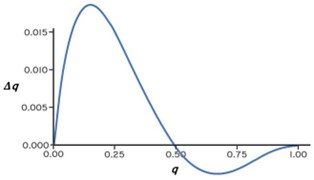
\includegraphics[width=0.65\textwidth,height=\textheight]{images/fig2-5.jpg}

}

\end{figure}

\end{tcolorbox}

\footnotetext{\(r = 0.47\); \(P = 0.04\) for log\textsubscript{10}
transformed data; \(N = 20\).}

\hypertarget{contrasting-the-ecological-hypotheses}{%
\chapter{Contrasting the Ecological
Hypotheses}\label{contrasting-the-ecological-hypotheses}}

\begin{figure}

{\centering 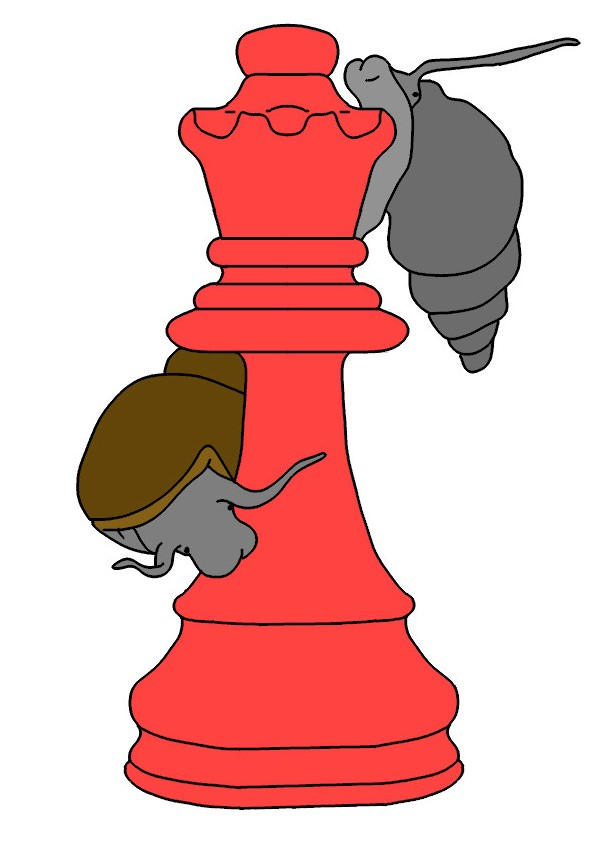
\includegraphics[width=0.4\textwidth,height=\textheight]{images/fig3-1.jpeg}

}

\end{figure}

As I mentioned in Chapter~\ref{sec-why-sex}, my dissertation focused on
intertidal communities. I was especially interested in how two different
barnacle morphs coexisted on rocky intertidal shores in the Northern
Gulf of California. I had initially assumed that the two types were
genetically determined and that they were likely to be different species
(Figure~\ref{fig-3-2}). However, after years of false starts,\footnote{I
  ran two years of field experiments designed to test for random
  settlement by genetically determined morphs. I also ran experiments
  designed to test for habitat selection by genetically determined
  morphs. The results were always negative. I finally tested for
  predator-induced development of the bent morph by placing
  \emph{Acanthina} snails in quadrats where juvenile barnacles had
  recently settled. I used herbivorous snails as a control. The results
  showed that the presence of \emph{Acanthina} induced development of
  the bent form, but the herbivorous snails did not. It was a thrilling
  discovery.} I found that one of the two morphs was induced by chemical
cues released by a predatory snail (Figure~\ref{fig-3-3}), and that the
induced morph was more resistant to attack by this predator (Lively
1986c).\footnote{Plasticity is more mainstream now than it was in the
  1980s. One reviewer of my paper was incredulous and recommended
  rejection from \emph{Evolution} because the bent morph was not
  ``genetically determined.'' The Associate Editor (John Endler)
  rejected the review and accepted the paper. Clearly, it is the
  developmental strategy that is genetically determined, not the morph
  per se (see also Lively et al.~2000, Hazel et al.~2004).} Hence, the
two morphs are not different species, but rather the result of
phenotypic plasticity. In a blink of a field season, I went from being a
community ecologist to an evolutionary biologist.

But why two morphs? Why didn't selection favor unconditional development
of the predator-resistant morph? Using predator-exclusion cages, I found
that predation was concentrated near crevices in the reef, which the
snails used during high tide as refuges (Lively 1986b). As the tide
receded, the snails moved out from these crevices onto the exposed rock
surfaces to forage on barnacles. When the tide returned, the snails
motored back to the crevices, presumably to hide from snail-crushing
rays that came in with the tide. This back-and-forth movement of snails
created high-predation zones near crevices and low-predation zones far
from crevices (about 20cm away). This finding explained why the
predation-resistant morph was almost always found near crevices. Field
experiments also showed that the predator-resistant morph grew more
slowly and was less fecund than the typical volcano-shaped morph (Lively
1986b). Hence there is a trade-off. Taken together, the results
suggested that plastic development was favored by natural selection to
survive in the high-predation zones (\protect\hyperlink{callout-3}{Box
3.1}). I would later come to think of adaptive plasticity as a type of
variation strategy. Sexual reproduction can also be seen as a type of
variation strategy (Lloyd 1984). And I was very fortunate to be able to
study sexual reproduction after moving to New Zealand.

\begin{figure}

\sidecaption{\label{fig-3-2}The two morphs of the intertidal barnacle,
\emph{Chthamalus anisopoma}. \textbf{Top}, the ``bent'' form is induced
by exposure to chemical cues released by a specialized barnacle
predator, the predatory gastropod \emph{Acanthina angelica}. The bent or
``hooded'' form reduces the risk of successful attack by this predator.
\textbf{Bottom}, the typical, conic form of the barnacle. The conic form
is more fecund per unit size, and it grows more rapidly than the bent
form, but it is also more susceptible to attack by the predator. Drawing
by ZMD.}

{\centering 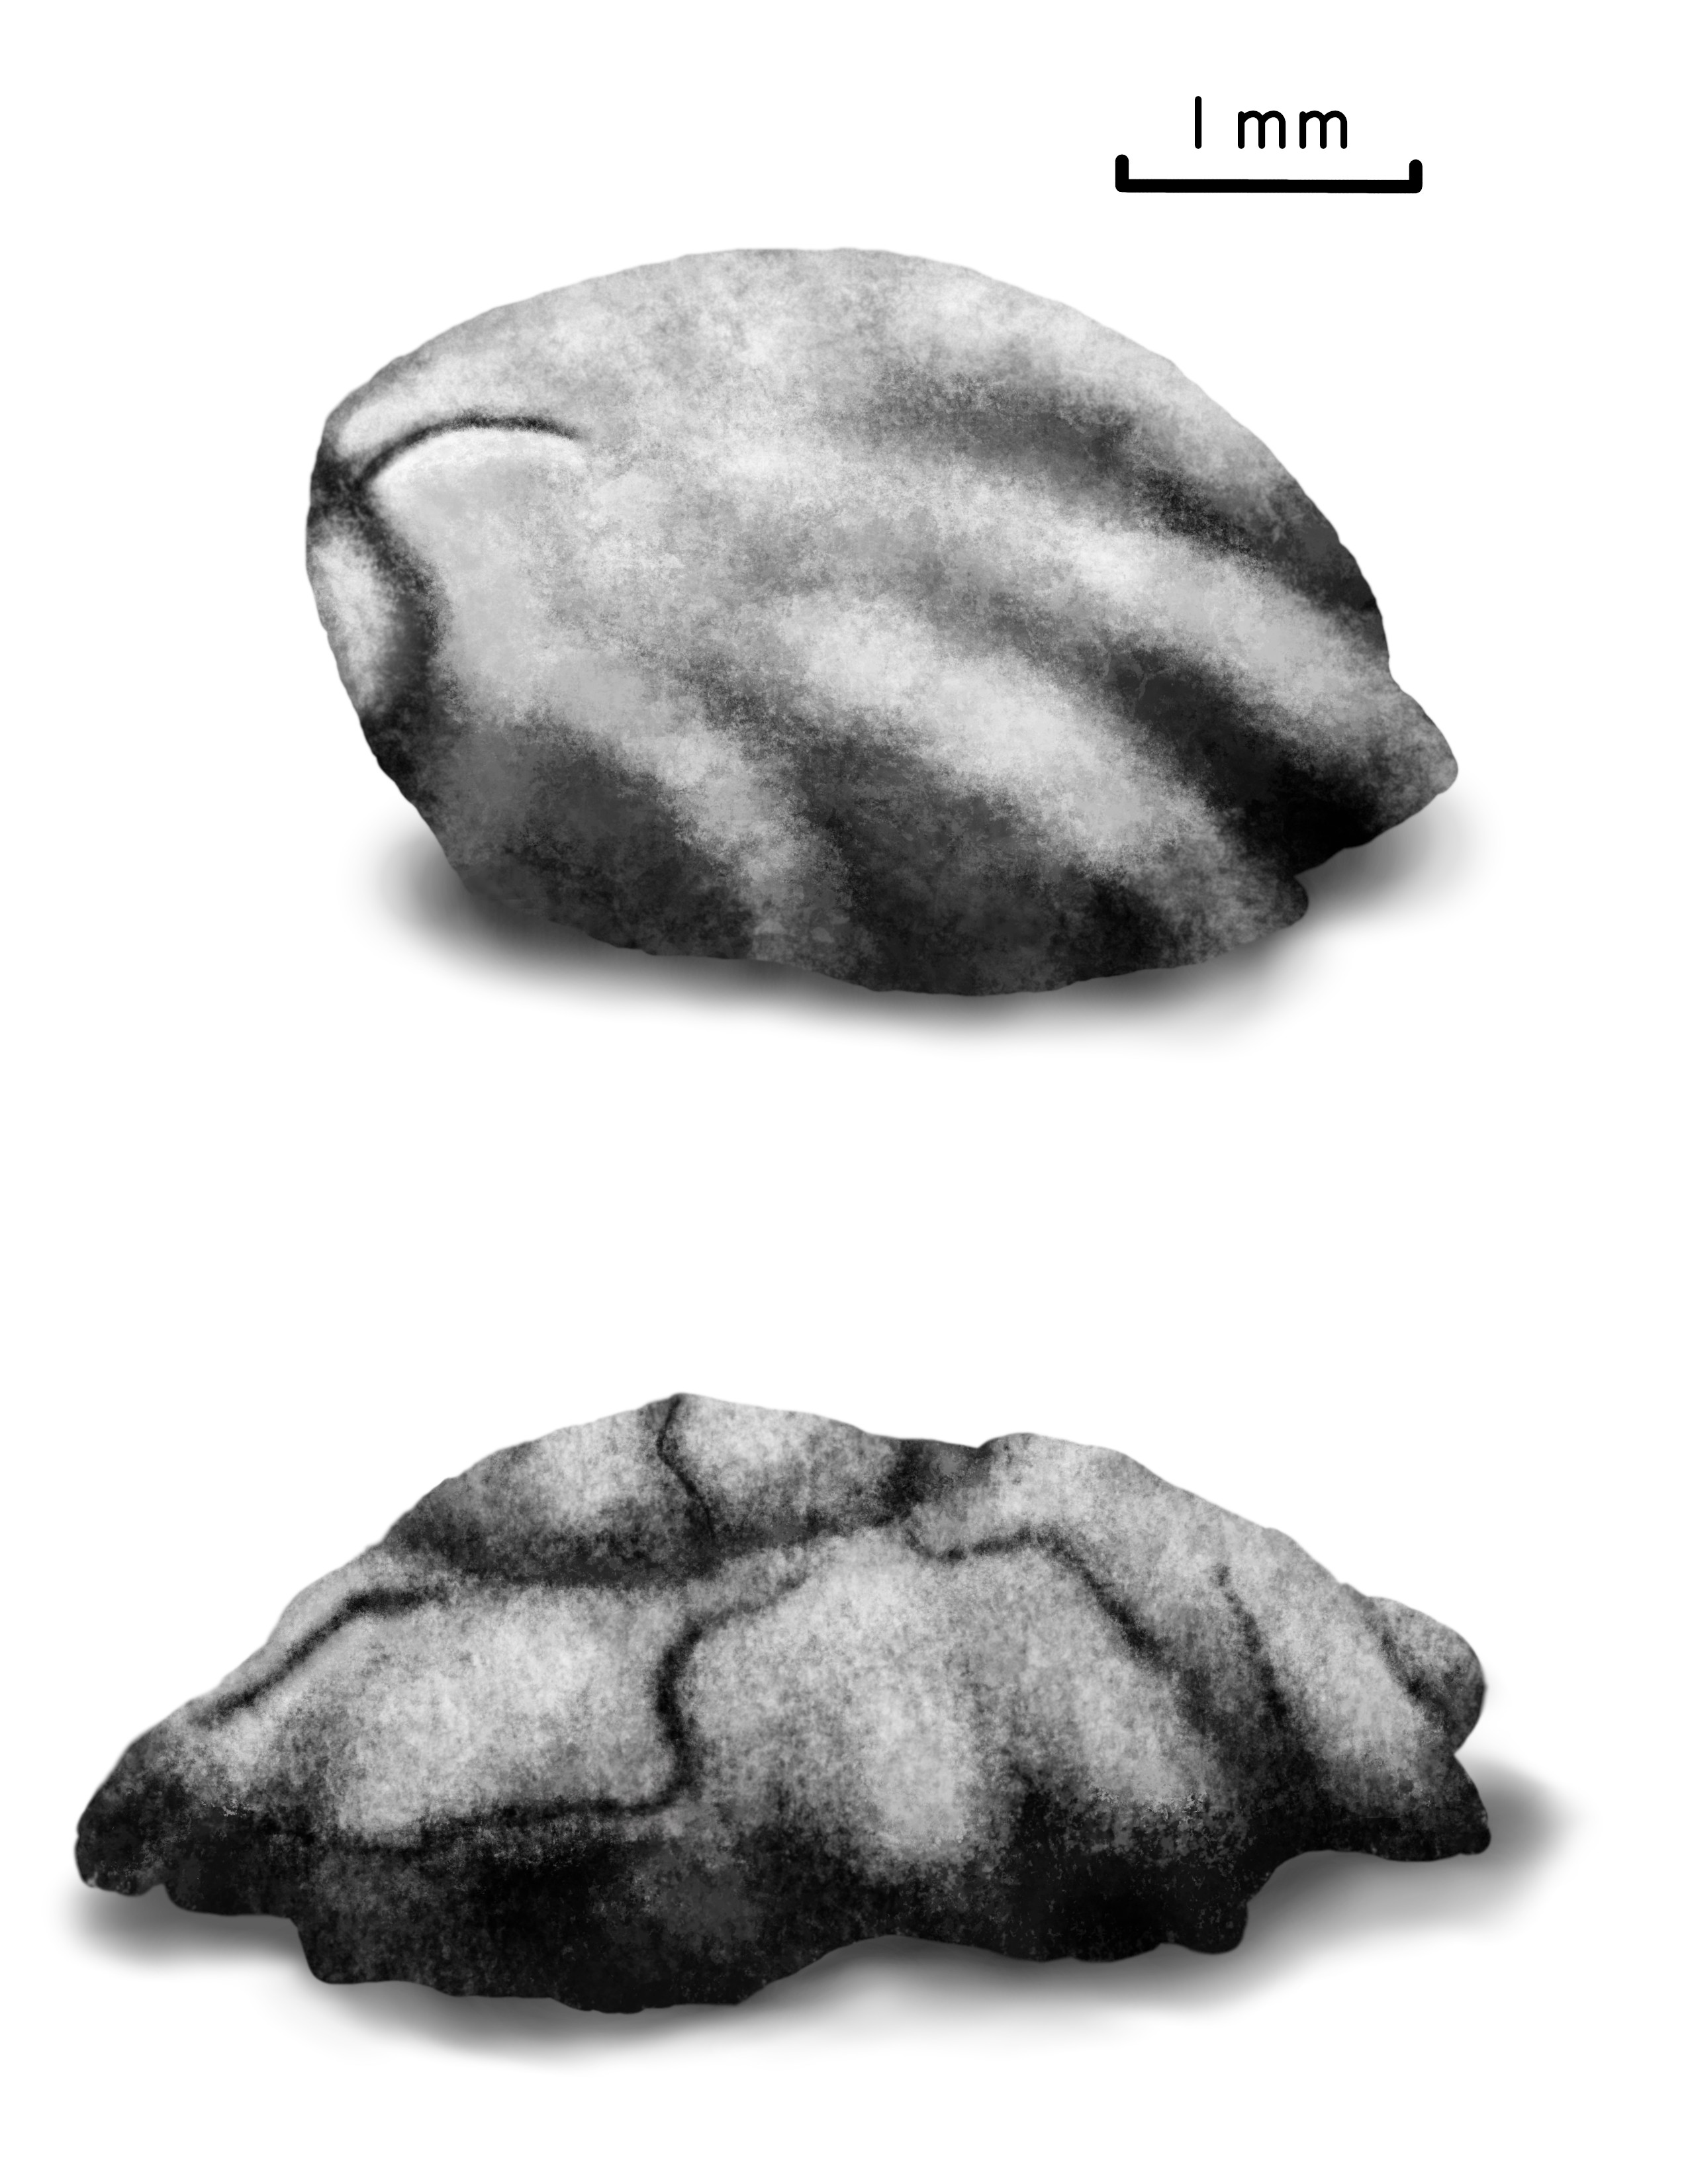
\includegraphics[width=0.4\textwidth,height=\textheight]{images/fig3-2.jpeg}

}

\end{figure}

\begin{figure}

\sidecaption{\label{fig-3-3}Line drawing of the predatory snail
\emph{Acanthina angelica} attacking the bent form of the barnacle. Note
that the predator has a spine on the outer margin of its shell. The
spine is used to push through the opercular plates of barnacles, and it
is very effective at penetrating and consuming the volcano-shaped form
of the barnacle. The bent form of the barnacle is more resistant to
attack of this kind because its aperture is less open to attack from
above. Drawing by ZMD.}

{\centering 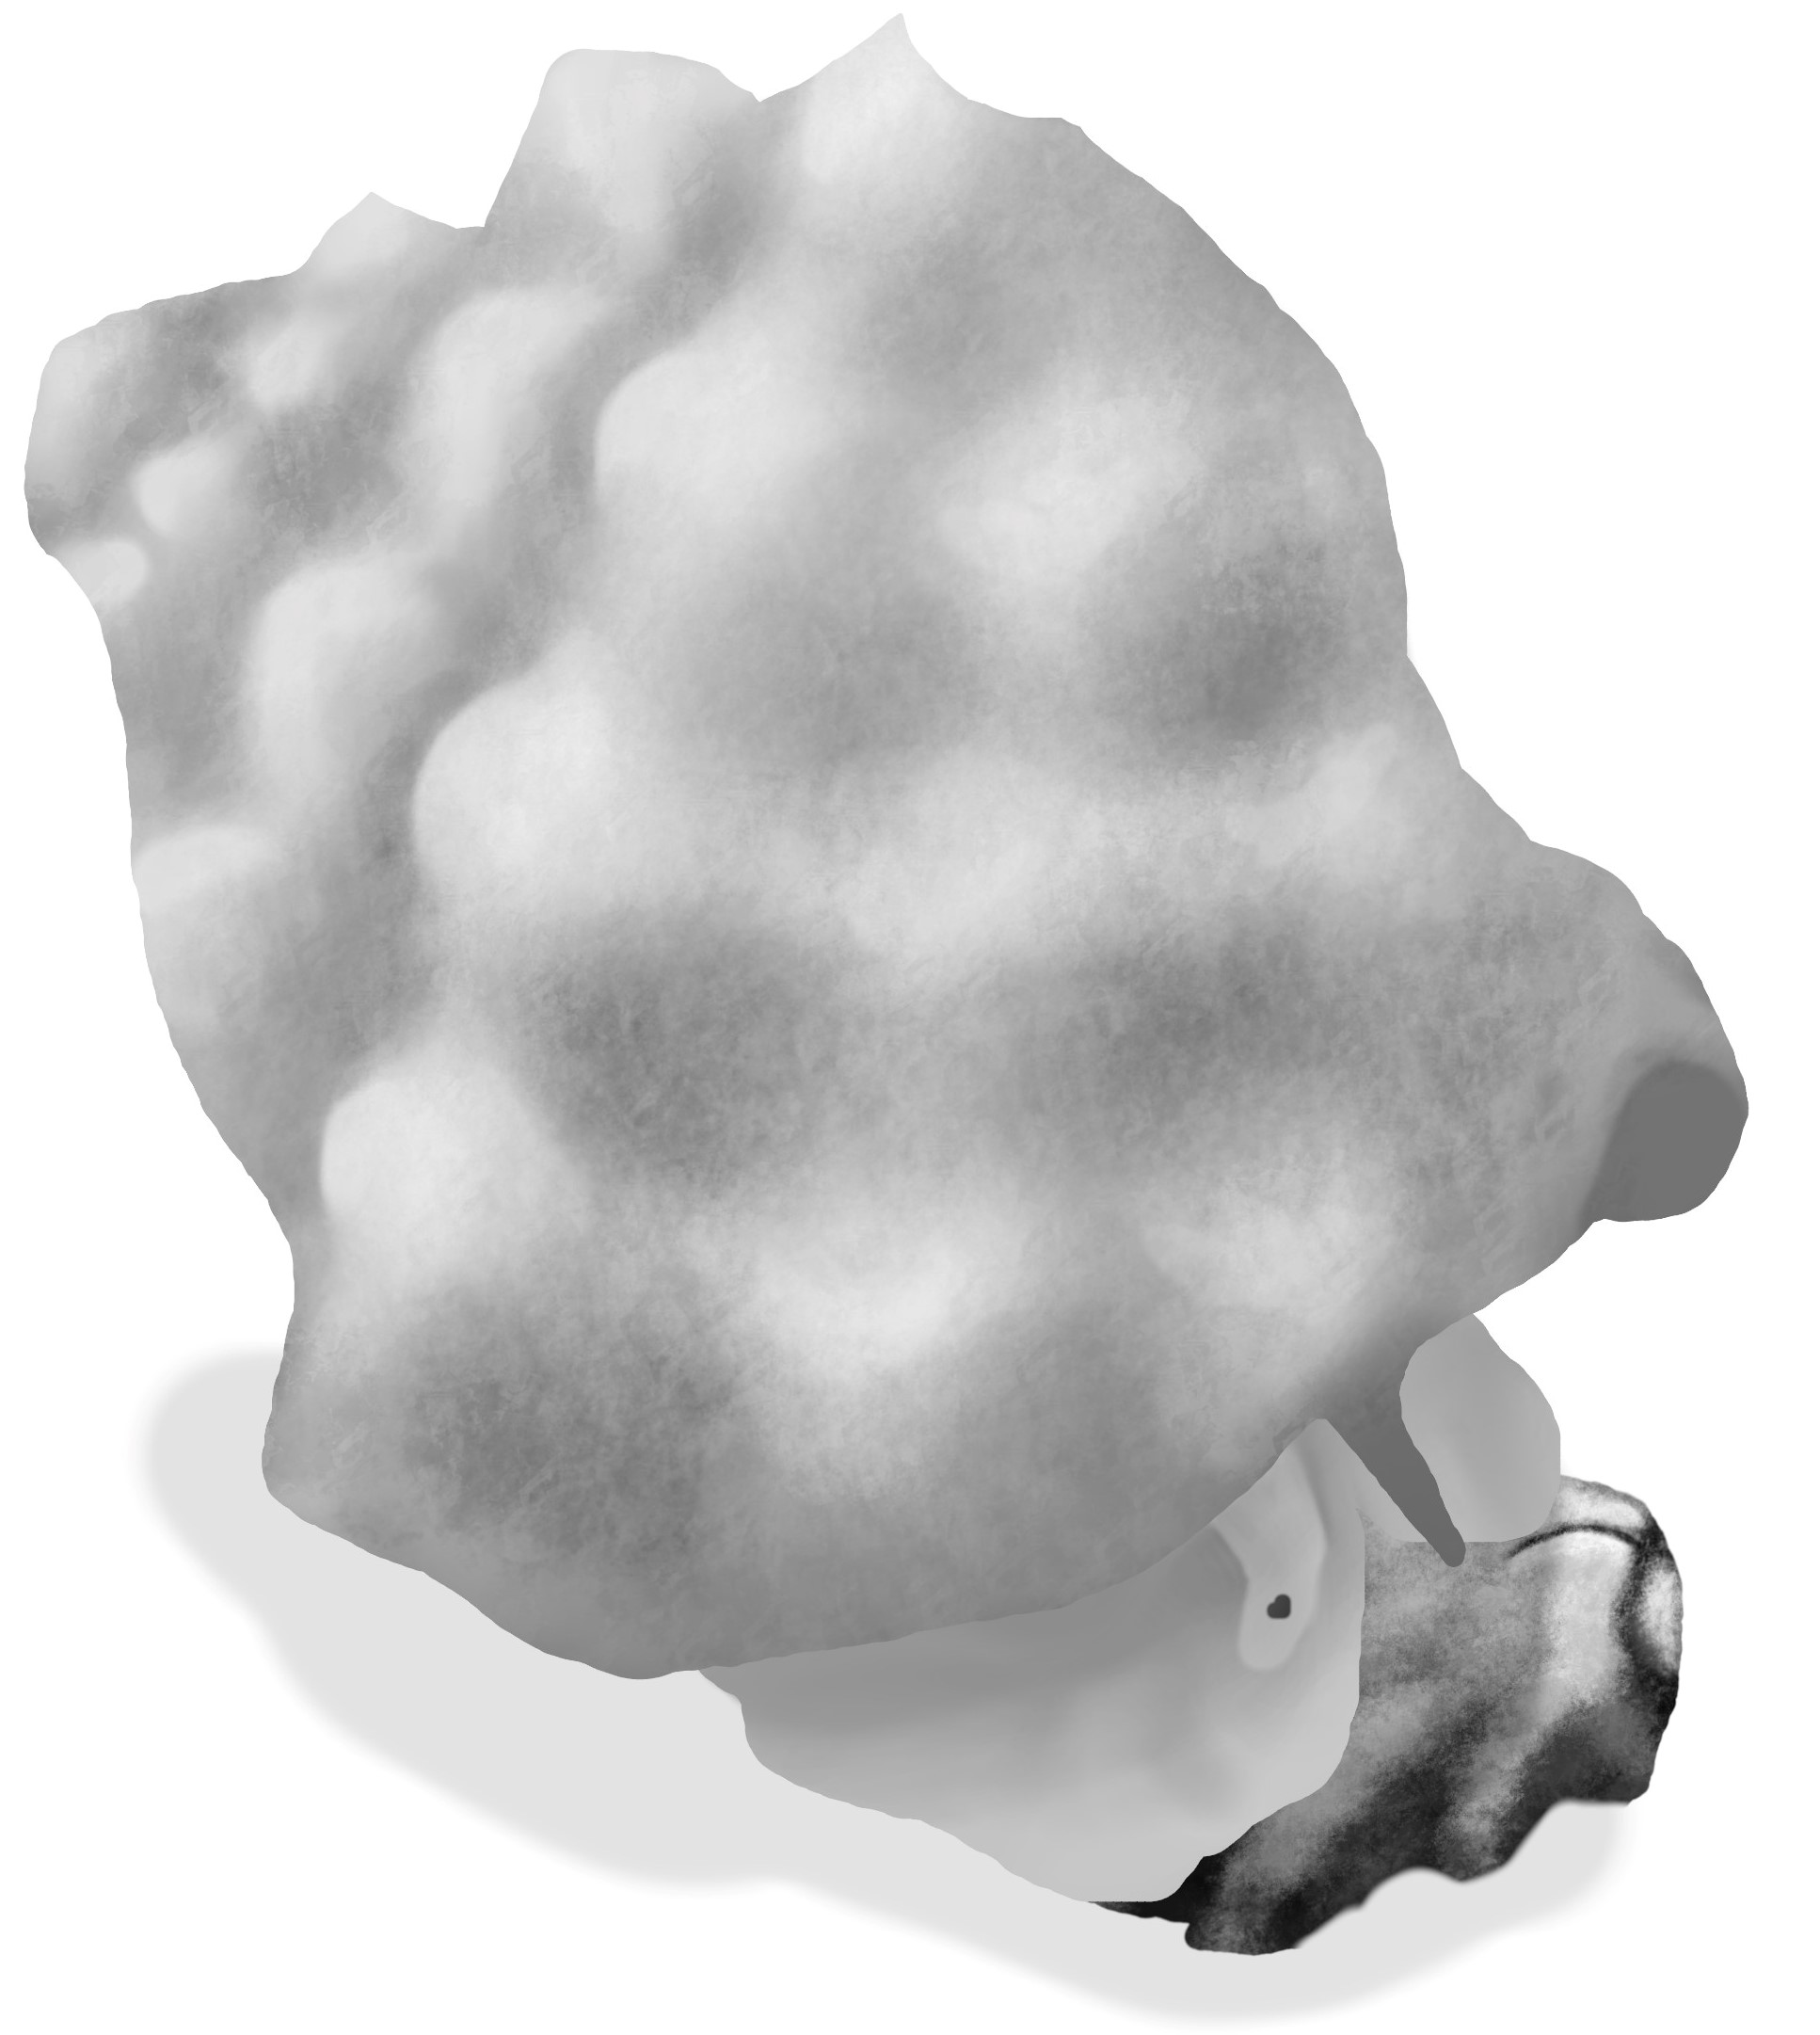
\includegraphics[width=0.4\textwidth,height=\textheight]{images/fig3-3.jpeg}

}

\end{figure}

I moved to New Zealand in 1984 just after defending my dissertation. My
reason for moving to New Zealand was simple: my spouse (Lynda Delph) was
there. Lynda had moved to New Zealand to study the evolution of plant
breeding systems with Prof.~David Lloyd. I did not have a job, but Lynda
had a small stipend from the Fulbright Foundation. By the time I moved
to New Zealand, we had only twelve dollars. But Lynda had found a flat
in a dormitory at the University of Canterbury, where she worked as a
``tutor.'' Tutors at the time were usually graduate students who served
as mentors for the resident students. We made many good friends during
our time as tutors, and it was a fascinating total immersion into Kiwi
culture. We did not have to pay rent, and we could eat for free in the
cafeteria. We could then spend Lynda's small Fulbright stipend on
sampling trips.

Then I got very lucky. I was awarded a three-year postdoctoral
fellowship from the NZ University Grants Committee. I had applied to
work on the evolution of facultatively parthenogenetic nematodes, which
represented a combination of my interests in developmental plasticity
and sex.\footnote{Facultative parthenogenesis is used to mean
  environmentally cued production of parthenogenetic females. I was
  originally planning to work on a nematode population that produced a
  mixture of sexual males and females at high density but only
  parthenogenetic females at low density.} These topics were also very
interesting to Wally Clark, a conceptual pioneer in the evolution of
plasticity. He was also head of the Zoology Department at the University
of Canterbury. I would not have received funding without the support of
Prof.~Clark. To my mind, the value of Clark's work remains
underestimated in general, but it had a big influence on me (e.g., Clark
1976).

I began looking for natural systems to study facultative
parthenogenesis.\footnote{We were trained ask questions first and then
  seek suitable organisms to address the questions. This was the
  tradition before model-systems research took over (Churchill 1997).}
To this end, I was reading Graham Bell's incredible book on the
evolution and genetics of sexual reproduction (Bell 1982). Searching the
index, I found a reference to \emph{Potamopyrgus antipodarum}, a New
Zealand freshwater snail. Bell had cited Mike Winterbourn's dissertation
work on this snail (Winterbourn 1970). Luckily for me, Prof.~Winterbourn
was just down the hall from me. I took the book to him, and I asked if
the snails were, in fact, facultatively parthenogenetic. He said no; the
snails were probably obligate asexuals, based on lab rearing experiments
that he had done. He also said that most populations were all female,
but some contained males. He then added that there was no obvious
pattern to the distribution of males. Amazing! I immediately decided to
work on these snails.\footnote{Prof.~Winterbourn was supportive of my
  work from this first day. He shared his knowledge of the snail system
  and of freshwater ecology, in general, with great enthusiasm. In
  addition, Mike met with my Ph.D.~students and took them into the
  field. This book would not have been possible without
  Prof.~Winterbourn.}

\hypertarget{the-method-of-multiple-working-hypotheses}{%
\section{The Method of Multiple Working
Hypotheses}\label{the-method-of-multiple-working-hypotheses}}

As graduate students at the University of Arizona, we read some of the
classics in the history and philosophy of science. Two of these papers
concerned the method of contrasting multiple working hypotheses
(Chamberlin 1890, Platt 1964).\footnote{See also Elliott and Brook
  (2007). They point out crucial differences between Chamberlin and
  Platt including that Chamberlin allowed for multiple ideas to be
  partially correct, which is important for Chapter~\ref{sec-chap6}.}
The idea is that multiple hypotheses should be simultaneously
considered. Then, to the extent possible, the alternatives are forced to
make different a priori predictions about the possible results. The hope
is that all but one of the alternative hypotheses would be eliminated,
leading to a ``strong inference'' that the remaining hypothesis is
supported (Platt 1964). Thus, the focus is on falsifying one or more of
the alternatives, rather than proving one of them (Popper 1959). Graham
Bell used this same method to contrast the ecological models for sex by
using data on the geographic distribution of asexual individuals across
many plant and animal taxa (Bell 1982). The data led him to reject the
Lottery Model (Chapter~\ref{sec-eco-hyp}). I decided to focus a similar
test directly on the New Zealand snails (Figure~\ref{fig-3-4}).

\begin{figure}

\sidecaption{\label{fig-3-4}The freshwater snail \emph{Potamopyrgus
antipodarum}. This small (3 -- 6 mm) prosobranch snail evolved from
marine ancestors (Phillips and Lambert 1990). Associated with the
invasion of freshwater, the snail evolved an internal brood pouch, where
the embryos hatch and develop before crawling out as juveniles. The
snail also evolved parthenogenetic reproduction. Parthenogenesis and
brooding are both rare traits in invertebrates, but they are often found
together (Lively and Johnson 1994). Some \emph{P. antipodarum}
populations presently consist of a mixture of diploid sexual individuals
and polyploid asexual females. The question under consideration here is,
why have the sexual females persisted in these mixed population snails?
What are the advantages of sexual reproduction? Photo credit: © Bart
Zijlstra / \href{}{www.bartzijlstra.com}.}

{\centering 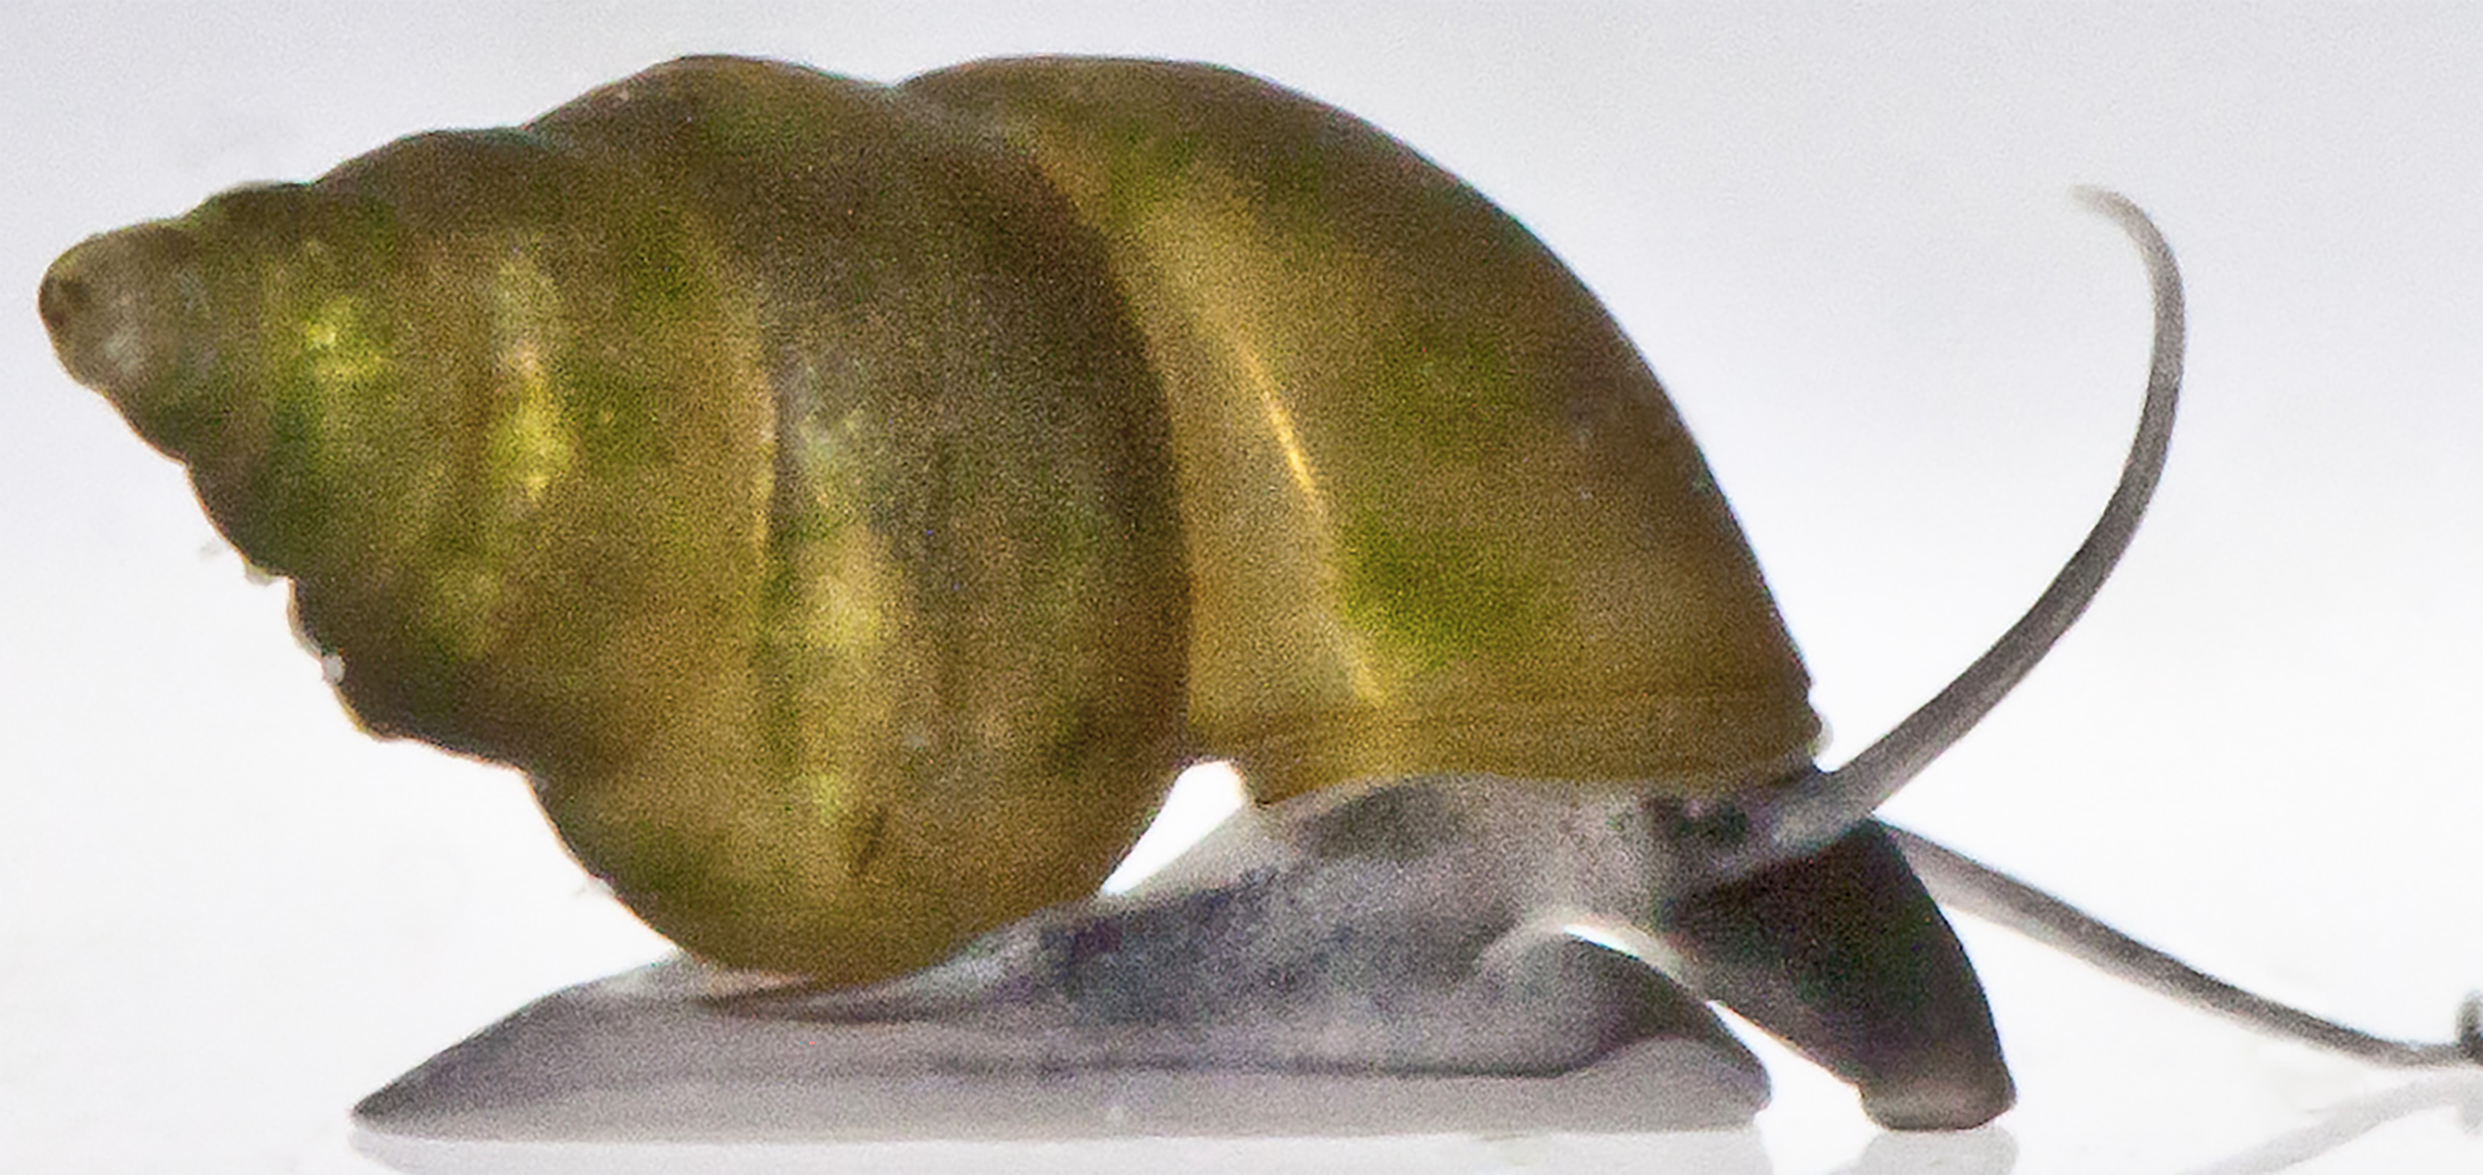
\includegraphics{images/fig3-4.png}

}

\end{figure}

The snails (\emph{Potamopyrgus antipodarum}) are often called mud
snails, but I think the term is a misnomer. They live on rocks and
vegetation in some of the most beautiful clear lakes, rivers, and
streams in New Zealand (``Potamo'' means river, not mud, in Greek). In
any case, based on Winterbourn's ecological work, streams seemed more
unstable than lakes, as water flow can vary dramatically, especially
during heavy rains in the mountains (Winterbourn et al.~1981). Hence,
under the Lottery Model, streams should have more sexual females (and
males) than lakes, because streams have more disturbance and less
competition (see Chapter~\ref{sec-eco-hyp} for a comparison of models).
By contrast, it seemed that competition for resources should be greater
in lakes than in streams. Indeed, lake populations of the snail can be
extremely dense. So, under the Tangled Bank, there should be more sexual
females in lakes, where competition for resources is expected to be
high. Finally, under the Red Queen Hypothesis, there should be more
sexual females where the risk of infection by coevolving parasites is
higher. As such, the different hypotheses could be forced to make
different predictions, with the important caveat that infection might be
correlated with habitat.

Some clarification regarding the prediction of the Red Queen Hypothesis
might be useful here. Some people have asked me why the correlation
between sex and infection is expected to be positive if, indeed,
parasites are the selective force for sexual reproduction. For example,
one could ask, if sex is so helpful in reducing infection risk, then
shouldn't the highly sexual populations have fewer, not more, parasites?
That could, of course, be expected in an experiment where hosts across
all populations were exposed to the same number of parasites. Then the
more genetically diverse populations with higher frequencies of sexual
females might be expected to have a lower prevalence of infection. But
it is not the case that all natural populations have the same risk of
infection. The idea under the Red Queen Hypothesis is that asexual
females would replace sexual females where the risk of infection is low,
and that sexual females would persist where the risk of infection is
high, provided that the parasites are highly virulent. That is how the
positive correlation could be generated. Nonetheless, the data could be
expected to be very messy, especially if the frequency of sex oscillates
over time in response to coevolutionary games with parasites.

The snails are infected by trematode worms, but I did not know anything
about trematodes when I first began dissecting snails. I was just
looking for males. Winterbourn told me that I would know a male snail
when I saw one, as they have a penis just behind the right tentacle. But
I had not observed any such structure on the many snails I collected
from the streams around the university. I was beginning to think that I
was missing something. Then one day, when I was dissecting a snail,
hundreds of swimming things came out. Sperm, I thought. My first male! I
took them to Wally Clark's research technician, Jan McKenzie, to put
under her fancy microscope. She informed me that sperm do not have eyes,
that they do not have spines on their tails, and that they are, in fact,
orders of magnitude smaller than these wiggling beasts under her lens.
She was not impressed. I had perfectly fit the Kiwi stereotype of North
American ecologists: good with statistics, but no knowledge of real
animals. She informed me that these swimming things were trematode
larvae, \textbf{sterilizing parasites} of snails. Happily, we remained
good friends, despite her disappointment in my training. And, I had
found my first infection, which meant that I might be able to test the
Red Queen.

Perhaps embarrassingly, I had a scientific bias against the Red Queen
going into the study. My bias was based on a study by May and Anderson
(1983). They showed that parasites had to kill infected individuals for
sex to be favored over asex in hosts. Parasites are usually not that
virulent; hence it seemed to me that parasites could not provide
sufficiently strong selection to \emph{generally} favor sex. I will
return to this important paper in another chapter and discuss how key
assumptions of their model have been relaxed.

\hypertarget{a-side-story-on-jms}{%
\subsection{A side story on JMS}\label{a-side-story-on-jms}}

John Maynard Smith (JMS) was one of the most influential theoretical
biologists in history of evolutionary thought. He was able to formulate
and communicate novel ideas with apparent ease. Around the time that I
was beginning to work on \emph{Potamopyrgus}, JMS came to New Zealand,
along with his wife, Sheila. He was invited by David Lloyd to spend time
at University of Canterbury and to deliver three public lectures, which
were all fantastic. During this time, JMS spent several weeks in New
Zealand. Lynda, David, and I were lucky enough to hang out with him
quite a bit. JMS was a remarkable individual. He could talk with anyone
and show a sincere interest in their work. One morning, I was sitting
next to JMS in the tearoom in the old Zoology Department. I was scared
speechless. He kindly asked me what I was working on, so I told him
about the snails. He knew of them! In fact, he had covered them in his
book, \emph{The Evolution of Sex}.\footnote{With respect to
  \emph{Potamopyrgus} (along with a parthenogenetic beetle) Maynard
  Smith (1978, page 65) wrote, ``Further Investigations of these cases
  could be most interesting.'' When I met JMS, I did not know (or did
  not remember) that he had written this. But I think that he was
  correct.} He was very excited that I was working on these creatures,
and he wanted to know my plan. I told him of my rough ideas for looking
at the distribution of males as a way of contrasting the ecological
hypotheses for sex. He looked directly at me, and said,``Interesting,
but I hope the answer is not parasites'' (or something like that). I
asked him, why not parasites? He laughed out loud, and with a big smile,
he said: ``Because Bill Hamilton thought of it first!'' I could tell he
was kidding. He then encouraged me to take the project on, and then he
laughed again and added: ``Whatever you do, don't go and solve the
problem of sex. Sex is too much bloody fun to have an answer!''

Toward the end of their time in New Zealand, JMS, Sheila, David, Lynda,
and I did a trip together around the South Island. The whole time was
incredible. Just listening to David and John talk about evolutionary
theory was a scientific dream. Towards the end of our trip, we were all
together in a restaurant at the Hermitage (near Mt. Cook) on the night
that JMS turned 65 and formally retired. Our server, a young alpinist
working to support his climbing in the Southern Alps, asked JMS, ``I
think that I saw a documentary about you. Are you famous?'' JMS (smiling
and intrigued) asked the alpinist what he remembered. Without
hesitation, the alpinist recited a perfect overview of evolution by
natural selection. JMS was clearly touched. Almost exactly half-way
around the world from Sussex England, in a small township in New
Zealand, JMS met someone whom he had influenced with his work. And this
was on the very night of his retirement.

The next day, we drove to a small lake near Mt. Cook that David knew
about: Lake Alexandrina. It was a glorious day, and we decided that we
might as well collect some snails. JMS waded into the water and
proceeded to collect a handful of \emph{Potamopyrgus} from the shallow
rocks. He handed the snails to me. He then laughed and said, ``When you
publish your study, I want to know the outcome for these exact snails.''
As it turned out, Lake Alexandrina has a mixed population of sexual and
asexual snails, and it has been the primary focus of our long-term
studies on \emph{Potamopyrgus}. The snail team still refers to this
original site of collection as ``JMS.'' Interestingly, JMS is one of the
most dynamic sites in the whole lake.

\hypertarget{the-distribution-of-male-snails}{%
\section{The Distribution of Male
Snails}\label{the-distribution-of-male-snails}}

To contrast the alternative ecological hypotheses, I sampled snails from
lakes and streams across the South Island of New Zealand. I could drive
Lynda's Volkswagen bug to most of the lakes, but I had to backpack into
many. Unfortunately, my time working in the Sonoran Desert had not
prepared me for the steep climbs, heavy rains, and chest-deep river
crossings on the South Island. I did not take enough food or dry clothes
on one trip, and my desert hiking boots disintegrated. I got my butt
kicked. But it was wonderful to have an excuse to see remote parts of
the South Island, especially after I got better gear and gained a better
understanding of the New Zealand bush.

I collected and dissected hundreds of snails from each of 29 streams and
22 lakes, mostly on the South Island. I recorded sex (male or female)
and infection by the trematodes that Winterbourn (1973) described. I
reasoned that the frequency of males in a population must be strongly
correlated with the frequency of sexual females simply because males are
only produced by sexual females.\footnote{This assumption turned out to
  be not strictly true. Polyploid females occasionally produce males,
  although they seem unlikely to be very fertile (Soper et al.~2013).}
The results showed that there were more males in lakes than in streams,
which was inconsistent with the Lottery Model, but it was consistent
with the Tangled Bank Model. However, male frequency was better
predicted by the frequency of trematode infection than by habitat
\emph{per se} (Lively 1987). Hence, surprisingly, the results favored
the Red Queen Hypothesis. I presented these findings to a small group at
David Lloyd's flat, and they convinced me to submit to \emph{Nature}
(Lively 1987).\footnote{The group included Mark McKone. Mark was a
  post-doc with David, and his comments were especially influential.
  Fifteen years later, I would become Ph.D.~advisor to one of Mark's
  star mentees at Carleton College, Maurine Neiman.}

A fascinating paper on the same topic was published in \emph{Nature} at
about the same time. This paper was also based on a strong-inference
test comparing the Red Queen and the Tangled Bank. The authors, Austin
Burt and Graham Bell, examined recombination in mammals (Burt and Bell
1987). They reasoned that under the Red Queen Hypothesis, longer-lived
mammals would have higher rates of recombination because more genetic
mixing would be favored as the asymmetry in host/parasite generation
time increased. In contrast, the Tangled Bank Model predicted that
shorter-lived mammals would have higher rates of recombination because
they have larger litters, and recombination might lead to reduced
competition among the more diverse offspring. Their results were
stunning. Recombination was tightly and positively related to longevity
in natural populations.\footnote{There we also some very interesting
  outliers. Domesticated mammals had very strong positive residuals for
  the rate of recombination. This result suggests that recombination was
  selected by frequent changes in the targets of artificial selection by
  humans.} The Red Queen was again supported.

Based on these studies in \emph{Nature}, I was beginning to think that
parasites might be a factor in selecting for cross-fertilization in
hosts. But my study as well as the study of Burt and Bell (1987) were
based on correlations. And every scientist knows that correlation is not
causation. On the other hand, these correlations were predicted \emph{a
priori} by Lloyd (1980) and others (e.g., Glesener and Tilman 1978, Bell
1982). The Red Queen was supported by the data, but the data were not
used to generate the hypothesis. Using the same data to both generate
and substantiate hypotheses is where the problem arises with
correlation, especially when multiple factors are considered in
``fishing expeditions.'' But forcing different hypotheses to make
different \emph{a priori} predictions about the direction of
correlations is, to my mind, a powerful way to evaluate alternatives.

As a brief aside, I cannot help but mention the human toll taken by R.A.
Fisher's use of ``correlation is not causation'' as a way to plant doubt
in the mind of smokers about the now-obvious risks of smoking (Gould
1991, Stolley 1991). Fisher was a consultant for the tobacco industry,
and he did the industry a great service at the cost of human lives. I
would also add that no test statistic is causation; F statistics derived
from analysis of variance are not causation. Causation might be inferred
from well-designed experiments, but no statistical test is causation.
Analytical theory is not causation either, as is well demonstrated by
the theoretical literature on sex/recombination. Causation instead may
be inferred when multiple independent lines of evidence point to similar
solutions. I think that Levins (1966) was correct when he wrote, ``Hence
our truth is the intersection of independent lies.\footnote{\begin{quote}
  Therefore, we attempt to treat the same problem with several
  alternative models each with different simplifications but with a
  common biological assumption. Then, if these models, despite their
  different assumptions, lead to similar results we have what we can
  call a robust theorem which is relatively free of the details of the
  model. Hence our truth is the intersection of independent lies (Levins
  1966).
  \end{quote}} Although he was referring specifically to mathematical
models, the same principle applies to biological systems. Ideally, the
multiple lines of evidence would include long-term field observations of
individual populations, broader biogeographic patterns across
populations, and direct experiments on multiple independent systems, as
well as multiple theoretical forays into the conditions under which the
hypothesis is expected to hold.

In any case, my view by 1987 was that the Red Queen Hypothesis merited
serious consideration.\footnote{I was also persuaded by elegant
  experimental studies on sweet vernal grass, which showed a
  density-independent advantage to having a rare genotype (Antonovics
  and Ellstrand 1984, Ellstrand and Antonovics 1985). Later studies
  showed that the rare advantage was likely due to escape from infection
  (Kelley et al.~1988, Kelley 1993, 1994).} For my own data, I now asked
whether the correlation between sex and infection was a ``red herring.''
In other words, could the correlation be generated because of something
else? Yes, it could. Here is how it might work. First, infection could
be higher in dense host populations as expected under theory (Anderson
and May 1979, May and Anderson 1979). Second, there might be more sex in
dense populations because asexual reproduction is favored in sparse
populations as a way for individuals to ensure reproduction even in the
absence of conspecific mates (Tomlinson 1966, Gerritsen 1980, Lloyd
1980). This latter idea is called the ``Reproductive Assurance
Hypothesis.'' Hence, one could find a positive correlation between sex
and infection as a simple consequence of epidemiology and selection for
reproductive assurance. So, I decided to sample again, this time
focusing on South Island lakes (Figure~\ref{fig-3-4} \&
Figure~\ref{fig-3-5}) while also collecting data on snail density. The
results were consistent with the epidemiological expectations, as there
was a marginally significant positive relationship between snail density
and infection prevalence, but there was no support for the Reproductive
Assurance Hypothesis (Lively 1992). Finally, the previously observed
positive relationship between sex and infection held
(Figure~\ref{fig-3-4}).\footnote{The partial correlation between percent
  male and prevalence of infection, while controlling for habitat, is
  highly significant (\(r = 0.36\), \(P < 0.001\)). However, the partial
  correlation between percent male and habitat, while controlling for
  prevalence of infection, is marginally significant (\(r = 0.21\),
  \(P = 0.05\)). Similar results were gained after males were excluded
  from the calculation of infection prevalence, which controls for any
  sex-specific differences in susceptibility (as shown in
  Figure~\ref{fig-3-4}); specifically, prevalence of infection in
  females was significantly correlated with male frequency while
  controlling for habitat (\(r = 0.37\), \(P < 0.001\)), but the
  converse was not true (\(r = 0.19\), \(P = 0.06\)).} The Red Queen was
still in the running.

\begin{figure}

\sidecaption{\label{fig-3-5}Results from surveys of New Zealand lakes
and streams showing percent males against the prevalence of female
infection by all species of trematodes. Note the upper left side of the
graph. There are no highly sexual populations where parasites are rare
or absent, which suggests that asexuals have replaced sexuals were
parasite-mediated selection is weak. This result is consistent with
Lloyd's prediction given in Chapter~\ref{sec-eco-hyp}. Circles represent
stream populations (Lively 1987) plus two river samples. Gray triangles
represent lake populations (Lively 1987). Black triangles represent lake
and tarn populations (Lively 1992). The correlation is positive and
statistically significant.}

{\centering 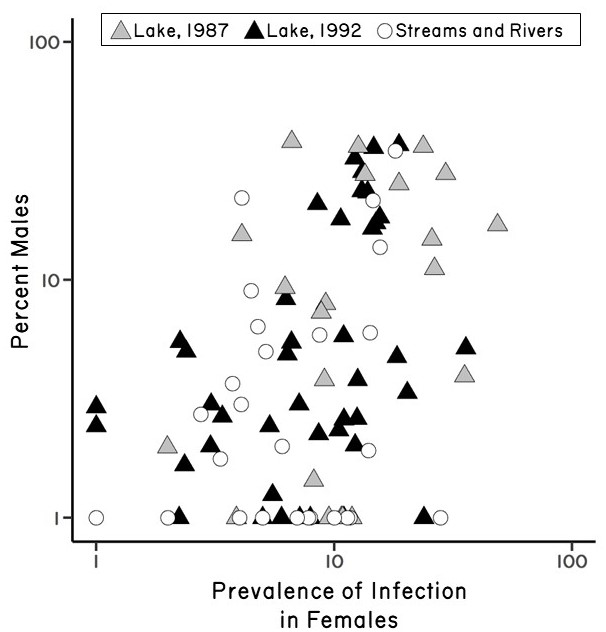
\includegraphics{images/fig3-5.JPG}

}

\end{figure}

These results suggested that parasite-mediated selection might
contribute to the persistence of sex in mixed populations of sexual and
asexual snails. It is of particular interest, perhaps, to note that
there are no populations with a high proportion of males in samples
where parasites were rare or absent (Figure~\ref{fig-3-5}). This finding
is consistent with David Lloyd's 1980 prediction that asexuals should
dominate in populations ``with a relaxation of biological hostility''
(see above). But the results are messy.

There are several reasons for why the results might be expected to be
messy. One is that prevalence of infection might not give a good
estimate of the strength of parasite-mediated selection (Lively 2001).
For example, infected snails might die at a faster rate than uninfected
snails because of the energetic demands of infection. In addition,
infected snails are more likely than uninfected snails to forage after
sunrise, which exposes them to predation by their final hosts, ducks
(Levri and Lively 1996, Levri and Fisher 2000). Prevalence of infection
might also fluctuate over time as the genetic diversity in the host
population changes and/or as the final hosts move among locations. We
now know that the prevalence of infection varies greatly among years and
among sites in the same lake (Gibson et al.~2016). Thus, detecting a
significant correlation between sex and infection could be dicey, even
if parasites were solely responsible for the short-term maintenance of
sex in mixed populations.\footnote{Using computer simulations, we
  recently found that detecting a significant positive correlation
  between clonal diversity and infection prevalence would only be
  expected in a fraction of parameter space, even when parasites were
  solely responsible for the maintenance of diversity (Lively et
  al.~2021).}

Along these lines, many of the points in Figure~\ref{fig-3-5} represent
a single sample taken at one site at one point in time. This limitation
likely introduces ``noise'' into the data, especially for samples where
parasites are only periodically common. For this reason, Jukka Jokela
and I selected 20 of the best sampled lakes from the data set given in
Figure~\ref{fig-3-5}.\footnote{In this smaller sample of 20 lakes, the
  correlation between male frequency and infection prevalence was
  positive but not statistically significant.} We resampled all 20 lakes
10 -- 15 years after my original samples. We found that prevalence of
infection was highly correlated between sample periods as was male
frequency (Lively and Jokela 2002). We then averaged the data for each
lake under the assumption that the averages would better represent both
the frequency of males and the prevalence of infection for each lake.
With these data, the correlation between male frequency and infection
prevalence was both positive and significant.\footnote{\(r = 0.47\);
  \(P = 0.04\) for log\textsubscript{10} transformed data; \(N = 20\).}

None of this is meant to imply proof of the Red Queen Hypothesis or that
density dependence and random environmental change are not relevant for
a full understanding of the problem.\footnote{I think density dependence
  is critically important. Disease transmission is certainly density
  dependent (Anderson and May 1979, May and Anderson 1979). Virulence
  may also be density dependent (Lively et al.~1995, Bell et al.~2006,
  Lively 2006). Habitat partitioning may also play a role in the
  distribution of sexual females among depth-stratified habitats
  (Negovetic and Jokela 2001).} But the results do imply that the Red
Queen Hypothesis was (and still is) worthy of further study.

\hypertarget{summary-2}{%
\section{Summary}\label{summary-2}}

\begin{enumerate}
\def\labelenumi{\arabic{enumi}.}
\item
  The co-occurrence of discrete morphs is inherently interesting to
  evolutionary biologists. Genetic diversity is also inherently
  interesting.
\item
  The New Zealand freshwater snail, \emph{Potamopyrgus antipodarum},
  some populations contain both sexual and asexual females. Other
  populations are mostly or completely parthenogenetic. This makes the
  snail a very useful natural system for contrasting alternative
  hypotheses for the maintenance of sexual reproduction.
\item
  The prevalence of sterilizing trematode larvae is a better predictor
  sexual reproduction in the snail than habitat (lakes vs.~streams),
  thus favoring the Red Queen Hypothesis over the alternative ecological
  hypotheses.
\item
  Comparing the \emph{a priori} predictions of multiple working
  hypotheses can be helpful to evaluate competing ideas. Field studies
  of natural systems may be required to fully understand why
  cross-fertilization is so common.
\end{enumerate}

\begin{figure}

\sidecaption{\label{fig-3-6}The distribution of male and female
\emph{Potamopyrgus antipodarum} across New Zealand. The percentage of
males is given in blue; the percentage of females is given in red. Pie
charts enclosed in boxes are for lakes and tarns that are very close
together. The large pie on the left-hand side shows the average
frequencies of males and females across all samples. (Redrawn from
(Lively 1992).)}

{\centering 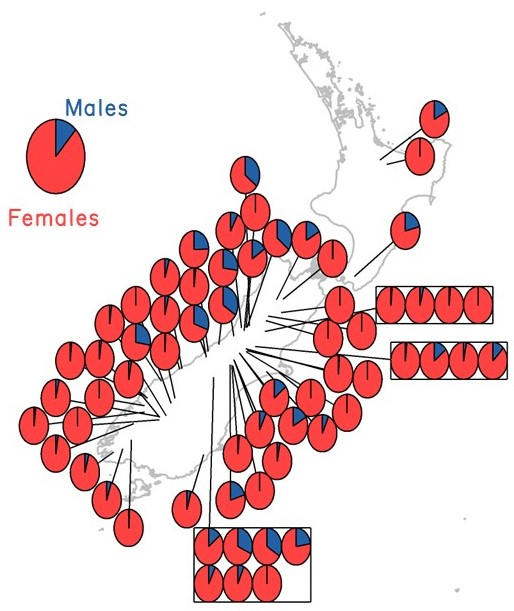
\includegraphics{images/fig3-6.JPG}

}

\end{figure}

\begin{tcolorbox}[enhanced jigsaw, left=2mm, bottomtitle=1mm, opacitybacktitle=0.6, breakable, leftrule=.75mm, coltitle=black, titlerule=0mm, opacityback=0, arc=.35mm, colback=white, title=\textcolor{quarto-callout-note-color}{\faInfo}\hspace{0.5em}{Box 3.1.}, toprule=.15mm, rightrule=.15mm, bottomrule=.15mm, colframe=quarto-callout-note-color-frame, toptitle=1mm, colbacktitle=quarto-callout-note-color!10!white]

As part of my dissertation research, I constructed a game-theoretic
model of selection on three strategies:

\begin{enumerate}
\def\labelenumi{\arabic{enumi}.}
\item
  canalized development into a high-fecundity morph,
\item
  canalized development to a low-fecundity, predation-resistant morph,
\item
  induced development into the low fecundity defended morph in the
  presence of predators.
\end{enumerate}

The model examined evolutionary stability for a range of frequencies for
two patches (high predation risk and low predation risk) across a range
of values for the accuracy of the cue predicting future predation risk
(Lively 1986a).

An example of the output is shown below. The results show that any of
the three strategies can be an ESS in part of the parameter
space.\footnotemark{} High reliability of the cue and intermediate patch
frequencies favor the plastic strategy. Genetic polymorphism is expected
under a relatively narrow set of conditions. Mixtures of constitutive
and plastic strategies can also be stable. Note that changing the patch
frequencies leads to evolutionary change. For example, reducing the
frequency of the low-risk patch can lead to a selective sweep (arrow a).
It can also lead to the evolution of plasticity (arrow b) and the
evolution of canalized development (arrow c). Increasing the accuracy of
the cue can also lead to the evolution of plasticity. It might be
especially interesting to note that the trajectory of arrow b would give
the appearance of saltatory change followed by stasis (i.e., punctuated
equilibrium) (Levinton 1988). Also note that the conditions for a
genetic polymorphism are relatively narrow. Redrawn from (Lively 1999b)
assuming a small cost to plasticity.

\begin{figure}[H]

{\centering 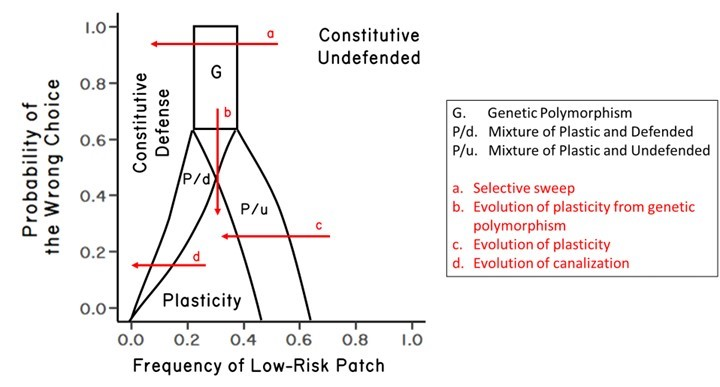
\includegraphics{images/fig3-7.JPG}

}

\end{figure}

\end{tcolorbox}

\footnotetext{``Parameter space'' represents all possible combinations
of variables as defined by the model. In
\protect\hyperlink{callout-4}{Box 3.1}, different strategies are favored
for different combinations of variables (i.e., different parts of the
parameter space).}

\hypertarget{sec-chap6}{%
\chapter{The Ratchet and the Red Queen}\label{sec-chap6}}

In 1988, Indiana University advertised for an assistant professor in
population biology, with emphasis on disease ecology. Lynda and I both
applied. Happily, we were offered a split position in Biology in which
we each got half salary. It may not sound like a good deal, but we were
thrilled. It is not easy for a dual-career couple in the same field. We
relocated to Bloomington in January of 1990, arriving during a cold snap
(-20\&degC). We moved into a university house; but we did not know
enough to have the electricity turned on before arrival. Luckily, we
still had our down sleeping bags, which we had purchased for field work
in the Southern Alps. Aside from the chilly start, moving to Bloomington
was the beginning of an academic dream come true. Most of this book aims
to highlight the work of my incredible students and colleagues at IU.

\hypertarget{the-problem-1}{%
\section{The Problem}\label{the-problem-1}}

\part{Back Matter}

\hypertarget{references}{%
\chapter*{References}\label{references}}
\addcontentsline{toc}{chapter}{References}

\markboth{References}{References}

\hypertarget{refs}{}
\begin{CSLReferences}{0}{0}
\end{CSLReferences}


\backmatter

\end{document}
